\documentclass[spanish]{article}

%%%%%%%%%%%%%%%%%%%%%%%%%%%%%%%%%%%%%%%%%%%%%%%%%%%%%%%%%%%%%%%%%%%%%%%%%%%%%%%%

% Language
\usepackage[spanish]{babel}

% Support for images
\usepackage{graphicx}

% Avoiding indenting of first paragraph's line.
\setlength{\parindent}{0cm}

% Support for hyperlinks.
\usepackage{hyperref}
\hypersetup {
        linktoc=all,
        hidelinks
}

% Additional section formatting.
\renewcommand\thesection{\arabic{section}}
\renewcommand\thesubsection{\thesection.\arabic{subsection}}

% Cover of the document
\title{Ingeniería de la usabilidad - Reto 2}
\author{Oussama Akachach Jouhrati\\[0.5cm]{\small Profesor/a: Mireia Ribera Turró}}
\date{\today}

%%%%%%%%%%%%%%%%%%%%%%%%%%%%%%%%%%%%%%%%%%%%%%%%%%%%%%%%%%%%%%%%%%%%%%%%%%%%%%%%

\begin{document}

\pagenumbering{gobble}
\maketitle
\newpage

\tableofcontents
\pagenumbering{arabic}
\setcounter{page}{2}
\newpage


% Customize from here.

\begin{abstract}

En este reto nos hemos centrado en la evaluación sin usuarios y el concepto
de arquitectura de la información, tras una previa lectura del
módulo 2 de la asignatura \textit{Métodos de evaluación sin usuarios}.
\newline

La primera actividad ha consistido en realizar una evaluación heurística
siguiendo los principios de Nielsen para la web de Freixenet y, seguido de ello,
hemos entregado una explicación breve de resumen de la evaluación heurística.
\newline

A continuación, se ha validado la accesibilidad de una página web de Freixenet,
siguiendo las indicaciones de la web del Consorcio World Wide Web. Para esta
pregunta, también se ha realizado un breve resumen de la evaluación de
accesibilidad.
\newline

Finalmente, para la parte de arquitectura de la información, se nos ha
solicitado hacer un esquema de la jerarquía de los productos dentro de
Freixenet y, por último, un test de estrés de navegación en el portal de visitas
de la misma página.
\newline

\end{abstract}
\newpage

\section{Pregunta 1}

\textbf{Jakob Nielsen es uno de los expertos más conocidos en el mundo de la
usabilidad. Usaremos 10 de sus principios heurísticos para ver si la web de
Freixenet los cumple. A partir de la lectura del material ``Métodos de
evaluación sin usuarios'' escrito por Mónica Zapata Lluch, dentro del Módulo 2.
\textit{Métodos de evaluación sin usuarios} realiza una evaluación heurística
según los diez principios heurísticos de Nielsen de la página web de Freixenet.
Puedes revisar también el método de la evaluación heurística en el Design
Toolkit de la UOC.}\newline

\textbf{\textit{Entrega una hoja de cálculo con la evaluación heurística en la que para
cada uno de los 10 principios debes poner ejemplos de cumplimiento o
incumplimiento midiendo su impacto (si afecta a muchos ususarios, si es crítico
para el proceso de compra...), la frecuencia (si los usuarios chocaran con ese
problema muy a menudo...) y observaciones. Te hemos facilitado una plantilla y
un ejemplo de evaluación heurística en los recursos de este reto. Entrega
también una explicación breve (1 página) de resumen de la evaluación
heurística.}}
\newline

En resumidas cuentas, lo que creemos que se ha tenido más en cuenta a la hora
de diseñar esta página es la forma, más que la función; la página se centra
mucho en proporcionar una presentación estética y agradable, pero descuida la
propia funcionalidad, o dicho de otra manera, el motivo por el cual la visitan,
que es acceder a los productos y ofertas que ofrecen. Esta página busca más
ser un anuncio un poco más interactivo que lo que se vería en televisión o en
un panel de la calle.\newline

Respecto a la evaluación heurística, destacamos la incapacidad de la página de
navegar de maneras menos tradicionales: mediante un lector de pantalla, el modo
de lectura del navegador, utilizando el teclado...\newline

Un aspecto realmente negativo que se ha encontrado ha sido el tener que ver
constantemente las pantallas de carga y las animaciones que, aunque hayamos
visitado la página, continuaban ejecutándose. Esto hace que la página se vea
mucho más lenta, que para el contenido existente, no es justificable. No lo
sería aunque tuviese una enciclopedia entera, teniendo en cuenta la potencia de
los dispositivos que tenemos hoy en día. Esto es debido a que, tanto por el
framework utilizado, como por el tamaño de los archivos, ralentizan demasiado la
visualización de la página. Este hecho es uno de los que más destacaríamos en
cuanto a crítica constructiva.\newline

\newpage

Sin duda, el mayor error que cometen es en los formularios de reserva, donde la
única validación de entrada que se hace es de los campos numéricos, siendo estos
el número de integrantes que van a acudir y el número de teléfono y, además, se
hace posterior a la operación de envío, por lo que el usuario/a deberá volver a
revisar la información introducida, campo por campo, hasta tenerlo todo en
orden.\newline

Además, el número de teléfono no está validado correctamente, ya que se ha
introducido en las pruebas el número de teléfono ``123'' y nos lo ha contado
como válido.\newline

Probablemente, la validación más importante que han descuidado es la del campo
``Fecha de visita''. Este campo es de tipo texto, pudiendo tenerlo como campo de
tipo fecha. La falta de esta validación invita a todo tipo de malentendidos e
información inprocesable.\newline

Por ejemplo, podemos encontrarnos con el caso de que haya un cliente americano
que utilice el formato mm/dd/yyyy, mientras que nosotros seguimos el formato
dd/mm/yyyy. Dando la libertad al usuario/a de escribir la fecha como le de la
gana puede dar pie a problemas en los que las reservas se hagan en días
diferentes a los esperados. Teniendo un campo fecha, este ya se encarga de que
cada uno visualice las fechas como espera, siguiendo la configuración del
navegador.\newline

\newpage

\section{Pregunta 2}

\textbf{Otro aspecto muy importante para el buen funcionamiento de la web es que
esté preparada para el uso que de ella harán las personas con alguna
discapacidad, es decir, que la web sea accesible. Puedes familiarizarte con el
concepto de accesibilidad con la guía del Design Toolkit de la UOC
``Accesibilidad''.}\newline

\textbf{Para validar la accesibilidad de un sitio web hay que seguir un proceso
largo y técnicamente complejo, en este reto haremos solo una pequeña
aproximación; por eso seguiremos la web del Consorcio World Wide Web ``Easy
Checks - A first review of web accessibility'' y te hemos facilitado un
formulario para hacer una primera evaluación del web.}\newline

\textbf{Analiza concretamente la sección de Freixenet ``Visita las
bodegas''.}\newline

\textbf{\textit{Entrega el formulario facilitado con tu evaluación. Entrega
también una explicación breve (1 página) de resumen de la evaluación de
accesibilidad.}}

\subsection{Formulario}

\subsubsection{Título de la página}

[CORRECTO] Ver si el título describe adecuada y brevemente el contenido de la
página.

\subsubsection{Alternativas textuales a las imágenes}

[INCORRECTO] Ver si cada imagen contiene un texto alternativo apropiado.

\subsubsection{Texto}

\textbf{Títulos}\newline

[CORRECTO] La página tiene un título.\newline

[CORRECTO] Todo el texto que parece un título está marcado como tal.\newline

[INCORRECTO] Todo el texto marcado como título es conceptualmente una sección de
título.\newline

[CORRECTO] La jerarquía de títulos tiene sentido. Idealmente, la página empieza
con un ``h1'' y no se salta niveles.\newline

\newpage

\textbf{Contraste}\newline

[INCORRECTO] La página debe tener un contraste mínimo de 4,5:1 para texto de
tamaño normal.\newline

\textbf{Ajuste de texto}\newline

[CORRECTO] Todo el texto se hace más grande.\newline

[CORRECTO] El texto no desaparece, ni se corta.\newline

[CORRECTO] El texto, las imágenes y otros contenidos no se solapan.\newline

[INCORRECTO] Todos los botones, campos de formulario y otros controles son
visibles y usables.\newline

[CORRECTO] El desplazamiento horizontal no es requerido para leer frases o
``bloques de texto''.

\subsubsection{Interacción}

\textbf{Acceso del teclado y enfoque visual}\newline

[INCORRECTO] Comprueba que se pueda tabular a todos los elementos, incluidos
enlaces, campos de formulario, botones y controles multimeda.\newline

[INCORRECTO] Comprueba que se pueda tabular fuera de todos los elementos a los
que se podía tabular.\newline

[INCORRECTO] Comprueba que el orden de tabulación sigue el orden lógico de
lectura.\newline

[INCORRECTO] Comprueba que el foco es claramente visible mientras tabulas sobre
los elementos.\newline

[INCORRECTO] Comprueba que puedas hacer todas las acciones con el teclado.\newline

[INCORRECTO] Comprueba que, al tabular en una lista desplegable, puedas usar las
flechas para navegar las opciones sin activar una acción.\newline

[INCORRECTO] Comprueba que cuando las imágenes sean enlaces, estas tengan un
foco claro y se puedan activar usando el teclado.\newline

\newpage

\textbf{Formularios, etiquetas y errores}\newline

[INCORRECTO] Comprueba que todos los elementos del formulario sean accesibles
siguiendo las indicaciones del acceso por teclado, incluyendo las listas
desplegables.\newline

[CORRECTO] Comprueba que las etiquetas estén posicionadas correctamente.\newline

[CORRECTO] Comprueba que los campos obligatorios estén marcados
claramente.\newline

[INCORRECTO] Comprueba que haya instrucciones para completar el formulario.\newline

[CORRECTO] Comprueba que exista una guía clara y específica para que el usuario
entienda y corrija el error.\newline

[CORRECTO] Comprueba que los errores sean fáciles de encontrar.\newline

[CORRECTO] Comprueba que los campos sin errores continúen poblados.

\subsubsection{General}

\textbf{Contenido en movimiento, parpadeante o intermitente}\newline

[CORRECTO] Comprueba si hay información en movimiento, que empiece
automáticamente y dure más de cinco segundos y, en caso de que exista, comprueba
que haya una manera de pausar, parar o esconder el movimiento.\newline

[CORRECTO] Comprueba si hay información que se actualice automáticamente y, en
caso de que exista, comprueba si hay una manera de pausar, parar o esconder la
información, o controlar la frecuencia de las actualizaciones.\newline

[CORRECTO] Comprueba que ningún contenido parpadea más de tres veces por
segundo.\newline

\textbf{Alternativas multimedia}\newline

\textit{No hay contenido multimedia en la página evaluada.}\newline

\newpage

\textbf{Comprobación de estructura básica}\newline

[INCORRECTO] Comprueba si la información de la página tiene sentido sin
imágenes, ni CSS.\newline

[INCORRECTO] Comprueba si el texto alternativo proporciona información adecuada
de las imágenes ausentes.\newline

[INCORRECTO] Comprueba si los bloques de información tienen títulos
claros.

\subsection{Comentario}

Esto ya se comentó en el primer reto, pero un detalle que considero que afecta
de manera considerable a la usabilidad de la página es la incapacidad de
navegarla mediante un lector de pantalla o el modo lectura del navegador. La
página está tan sobrecargada de contenidos, probablemente, por el framework
utilizado para desarrollar el frontend, que gran parte del contenido acaba
desapareciendo si utilizamos dicha función.\newline

Si le sumamos esto a que no se puede navegar por el teclado y que los botones
``Call to action'' están escondidos en bloques de texto, los títulos de los
cuales tienen el mismo color que los enlaces, da como resultado una navegación
bastante poco placentera.\newline

Visualmente, la página es atractiva. Mantiene un diseño minimalista, centrado en
el contenido, pero luego comete errores de usabilidad bastante graves que
afectan a la experiencia general.\newline

Otro detalle que se comentó en el reto pasado fue el caso del contraste, siendo
este bastante pobre. Inicialmente, vimos como el amarillo con el blanco era
difícil de leer y, la letra, al ser tan pequeña, añadía más esfuerzo a
comprender qué es lo que ofrecía la página. Con la extensión de Firefox del
cálculo de contrastes, hemos podido ver que incluso los textos de letra oscura
frente a fondo blanco, como puede ser el caso de la descripción de las
experiencias, tienen un contraste inadecuado, según estas indicaciones.\newline

El punto más negativo de la página es algo que ya se ha comentado en la primera
pregunta de este reto y, es que el formulario de reservas tiene una validación
de entrada bastante deficiente. Este sólo valida, tras pulsar el botón de
enviar, los campos de tipo número, incluyendo el teléfono móvil de la persona
que realiza la reserva. Esto significa que la validación del teléfono no sigue
ninguna expresión regular y que, con ser un número, ya se da por válido.\newline

\newpage

El correo electrónico se valida correctamente, pero el campo más importante y,
sorprendentemente, no validado, es el campo de fecha de visita. Se puede
introducir lo que uno quiera, puesto que está configurado como un campo de tipo
texto. Se requiere urgentemente cambiar a uno de tipo fecha, para evitar llenar
la base de datos del sistema de registros indeseados.\newline

Como punto positivo, también podemos añadir que la página a valorar no tiene
vídeos reproduciéndose constantemente, ni animaciones en exceso, exceptuando el
claro error de esconder los botones ``Call to action'' y mostrarlos sólo cuando
el usuario pasa el ratón por encima de los bloques de experiencias.\newline

En definitiva, a menos que se busque navegar de una manera tan específica como
en un navegador web de un ordenador, exlcusivamente con el ratón, esta página se
vuelve inefectiva para su uso.\newline

\newpage

\section{Pregunta 3}

\textbf{Finalmente analizaremos la navegación por dentro de la web. Haz un
esquema de la jerarquía de los productos dentro de Freixenet.}\newline

\textbf{La disciplina que trata de como organizar los contenidos en una web se
denomina ``Arquitectura de la información''. Te puedes familiarizar con este
concepto en el libro de Rosenfeld, Morville y Arango que encontrarás en la
sección de recursos.}\newline

\textbf{Además del esquema jerárquico de los productos, realiza también el test
de estrés de navegación en el portal de visitas. Identifica claramente cada una
de las secciones que se piden. En el caso de estudio podrás encontrar un ejemplo
de su aplicación.}\newline

\textbf{\textit{Entrega el esquema de categorías, dentro de la sección de
visitas de Freixenet. Harás el esquema general y solo desarrollarás esta
sección. Entrega también los resultados del test de estrés de la misma página
con una indicación clara de las secciones identificadas.}}\newline

\subsection{Esquema de la jerarquía de los productos}

\textbf{Página: Enoturismo}

\begin{itemize}

        \item Visita las bodegas
        \begin{itemize}

                \item Cava Bar
                \item Freixenet tour
                \item Visitas \& maridaje
                \item Visitas combinadas

        \end{itemize}
        \item Experiencias enogastronómicas
        \item Actividades enoturísticas
        \item Eventos

\end{itemize}

\newpage

\subsection{Test de estrés}

\subsubsection{¿De qué va esta página?}

\begin{center}
        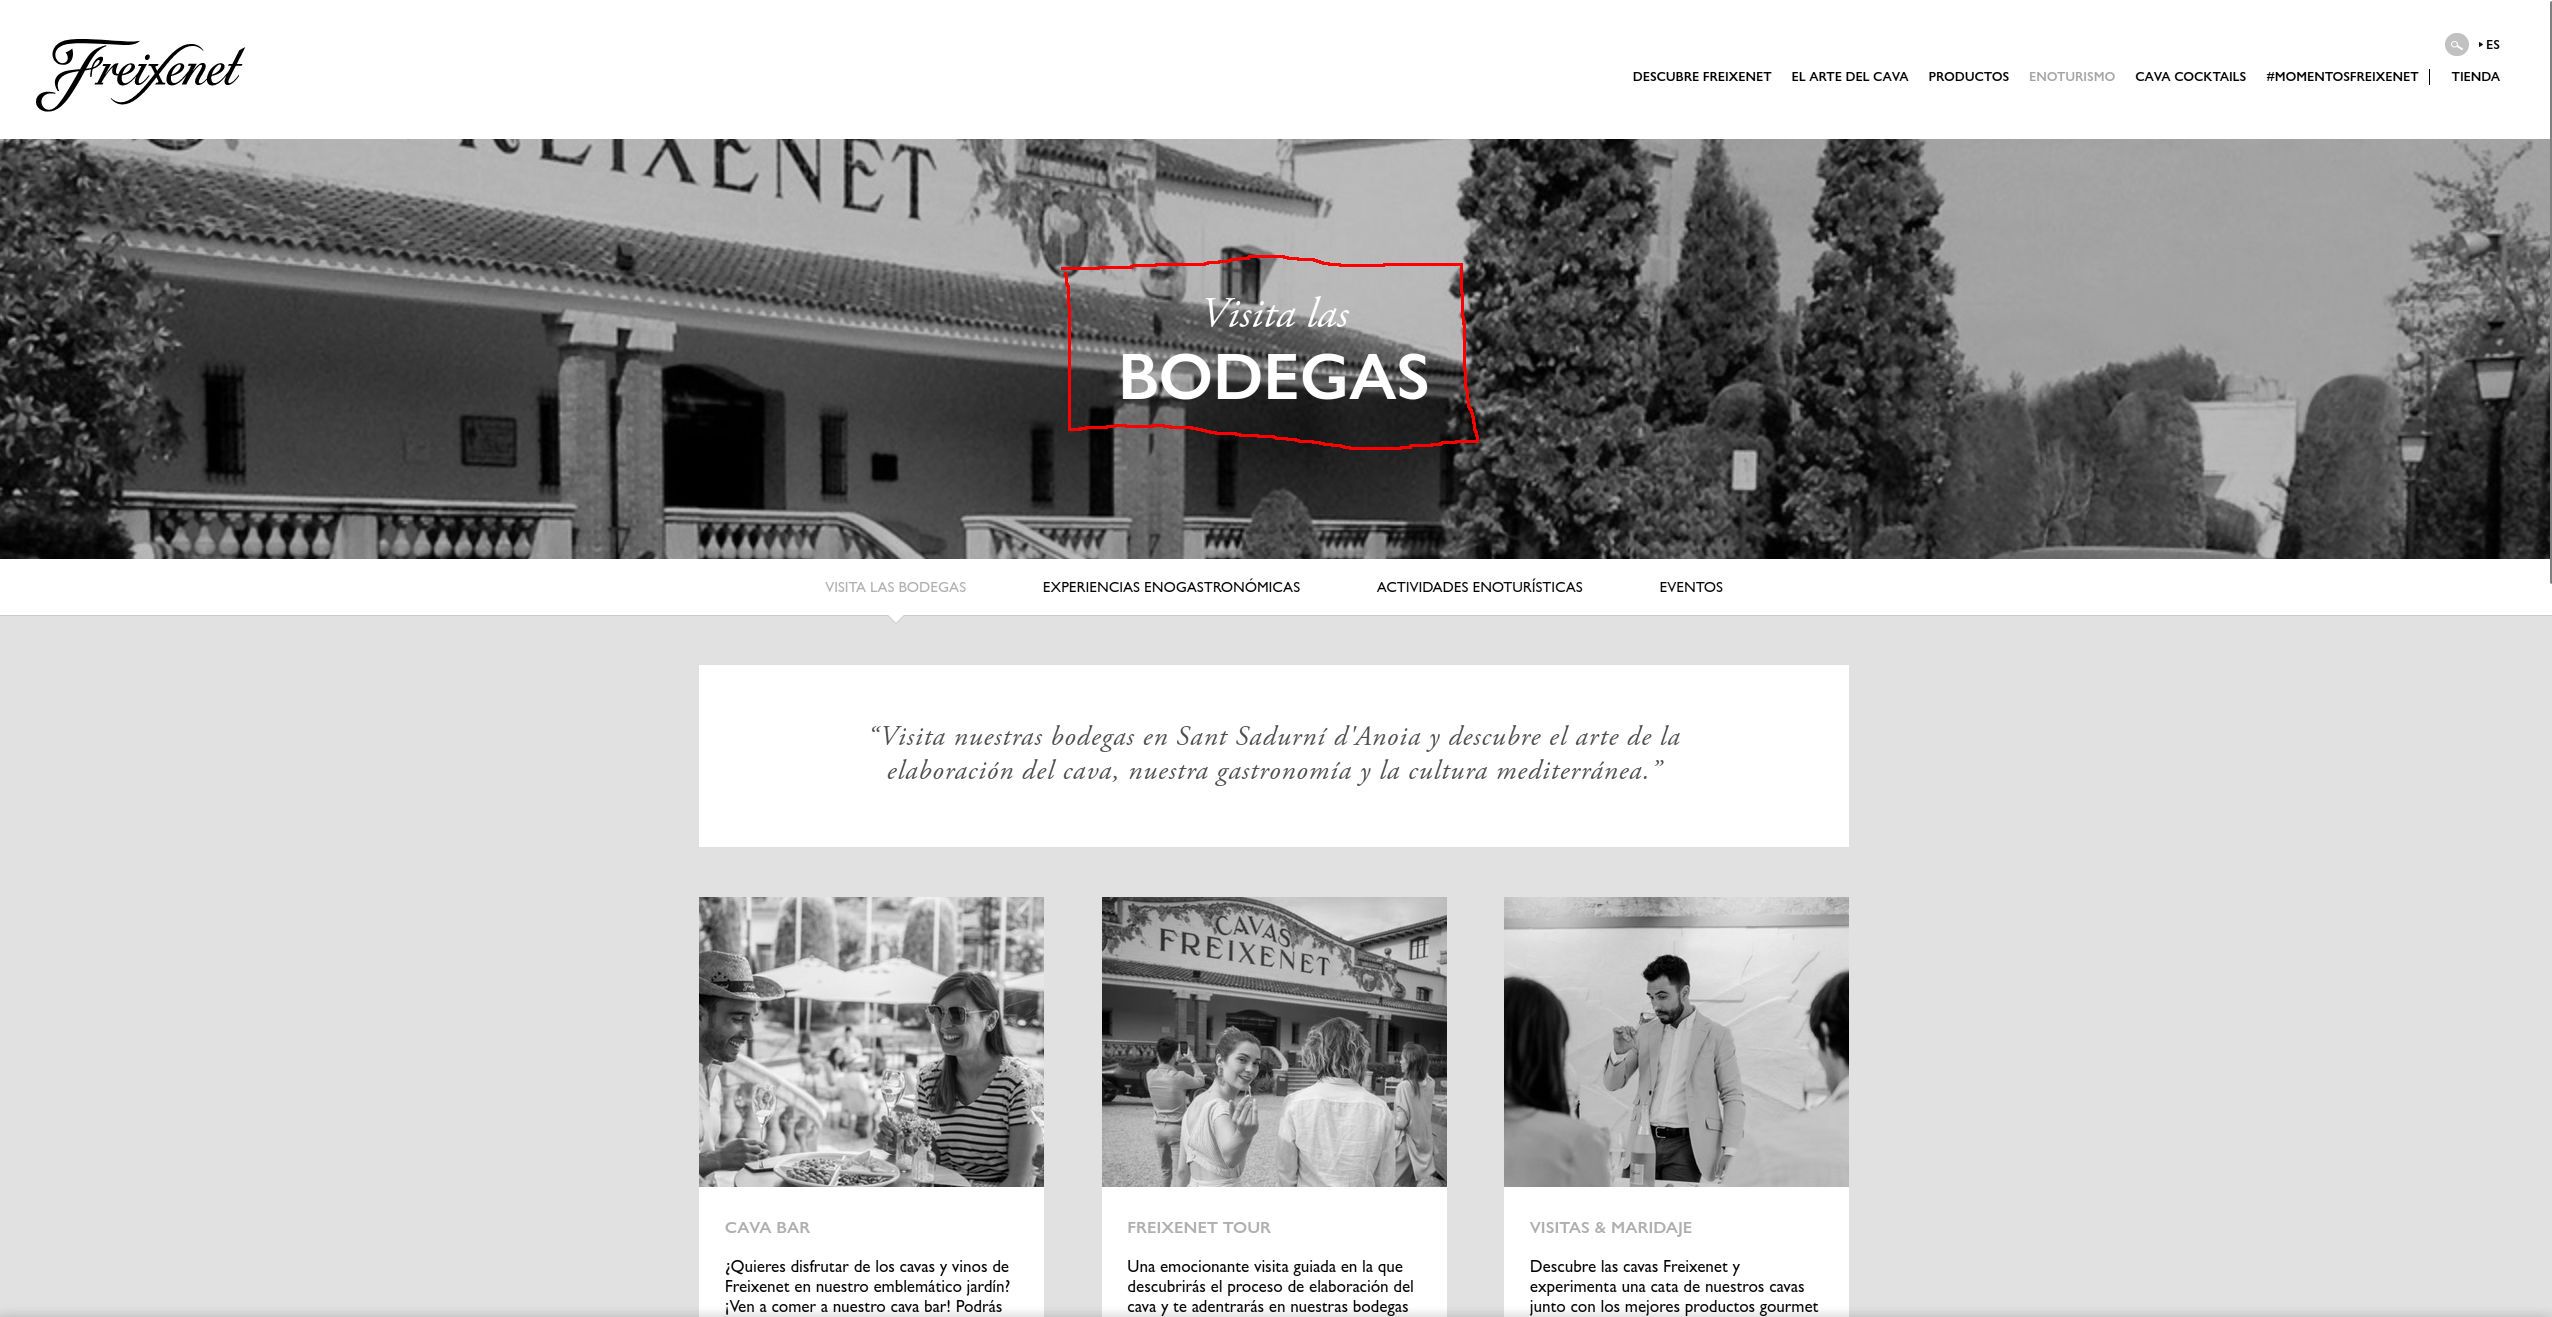
\includegraphics[scale=.1]{../img/1.png}
\end{center}

\subsubsection{¿Qué página es esta?}

\begin{center}
        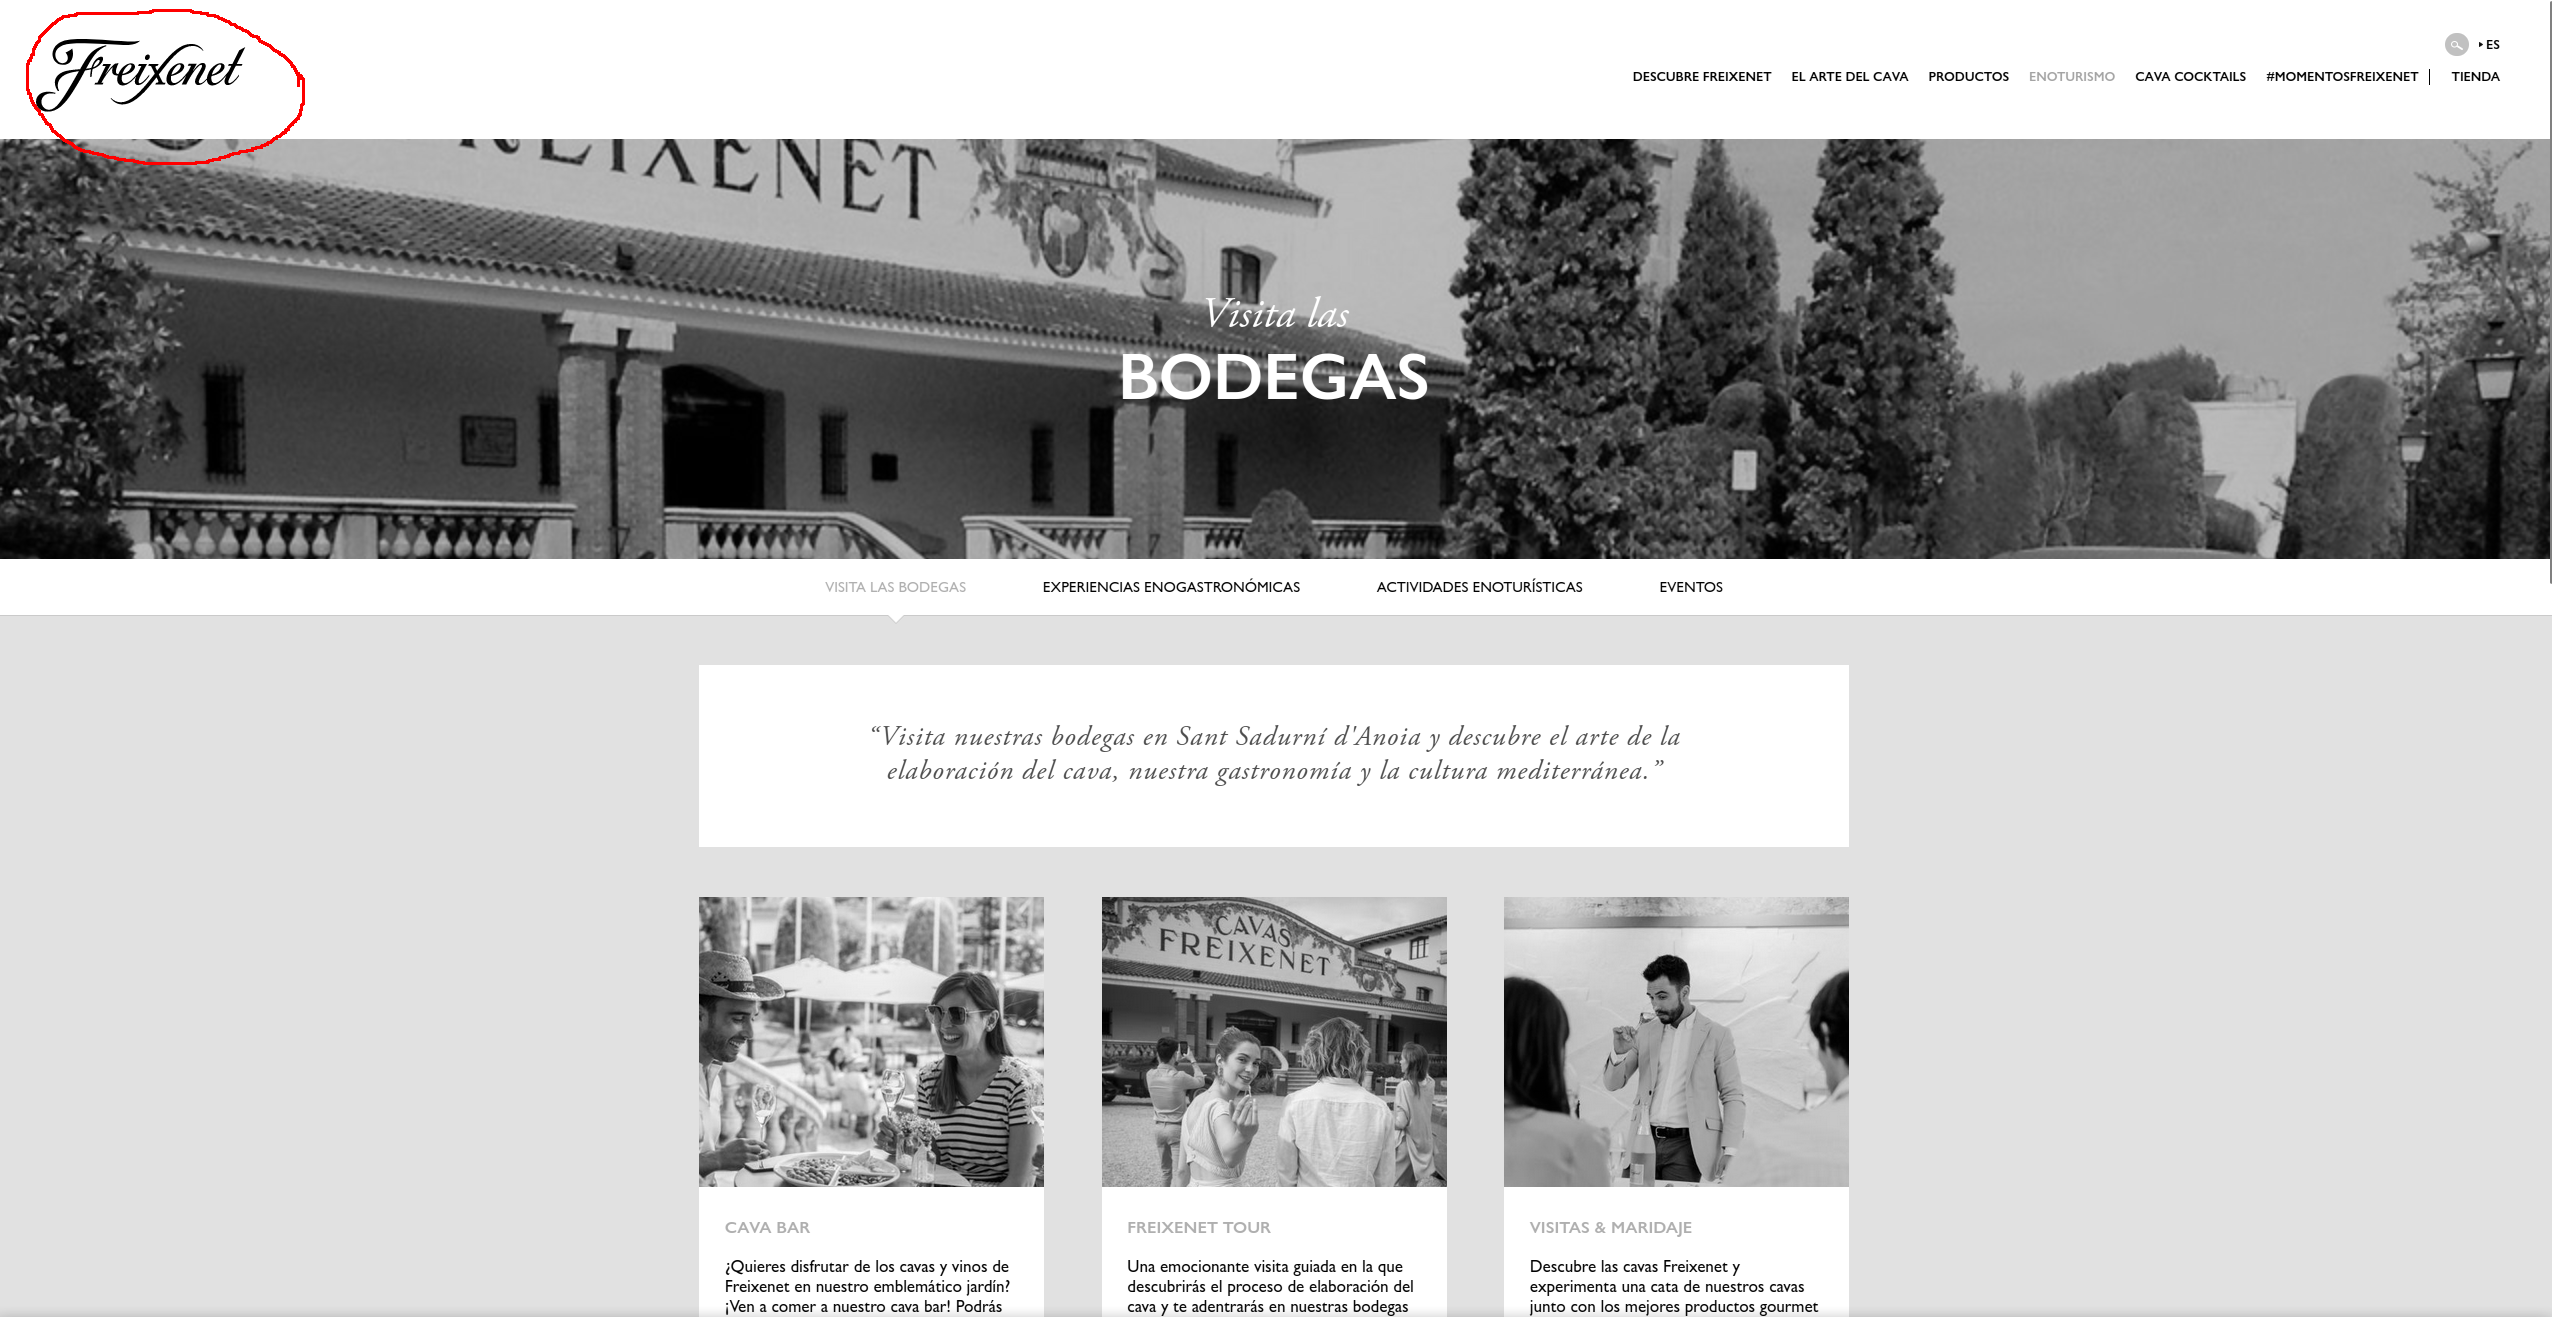
\includegraphics[scale=.1]{../img/2.png}
\end{center}

\subsubsection{¿Cuáles son las secciones principales de esta página?}

\begin{center}
        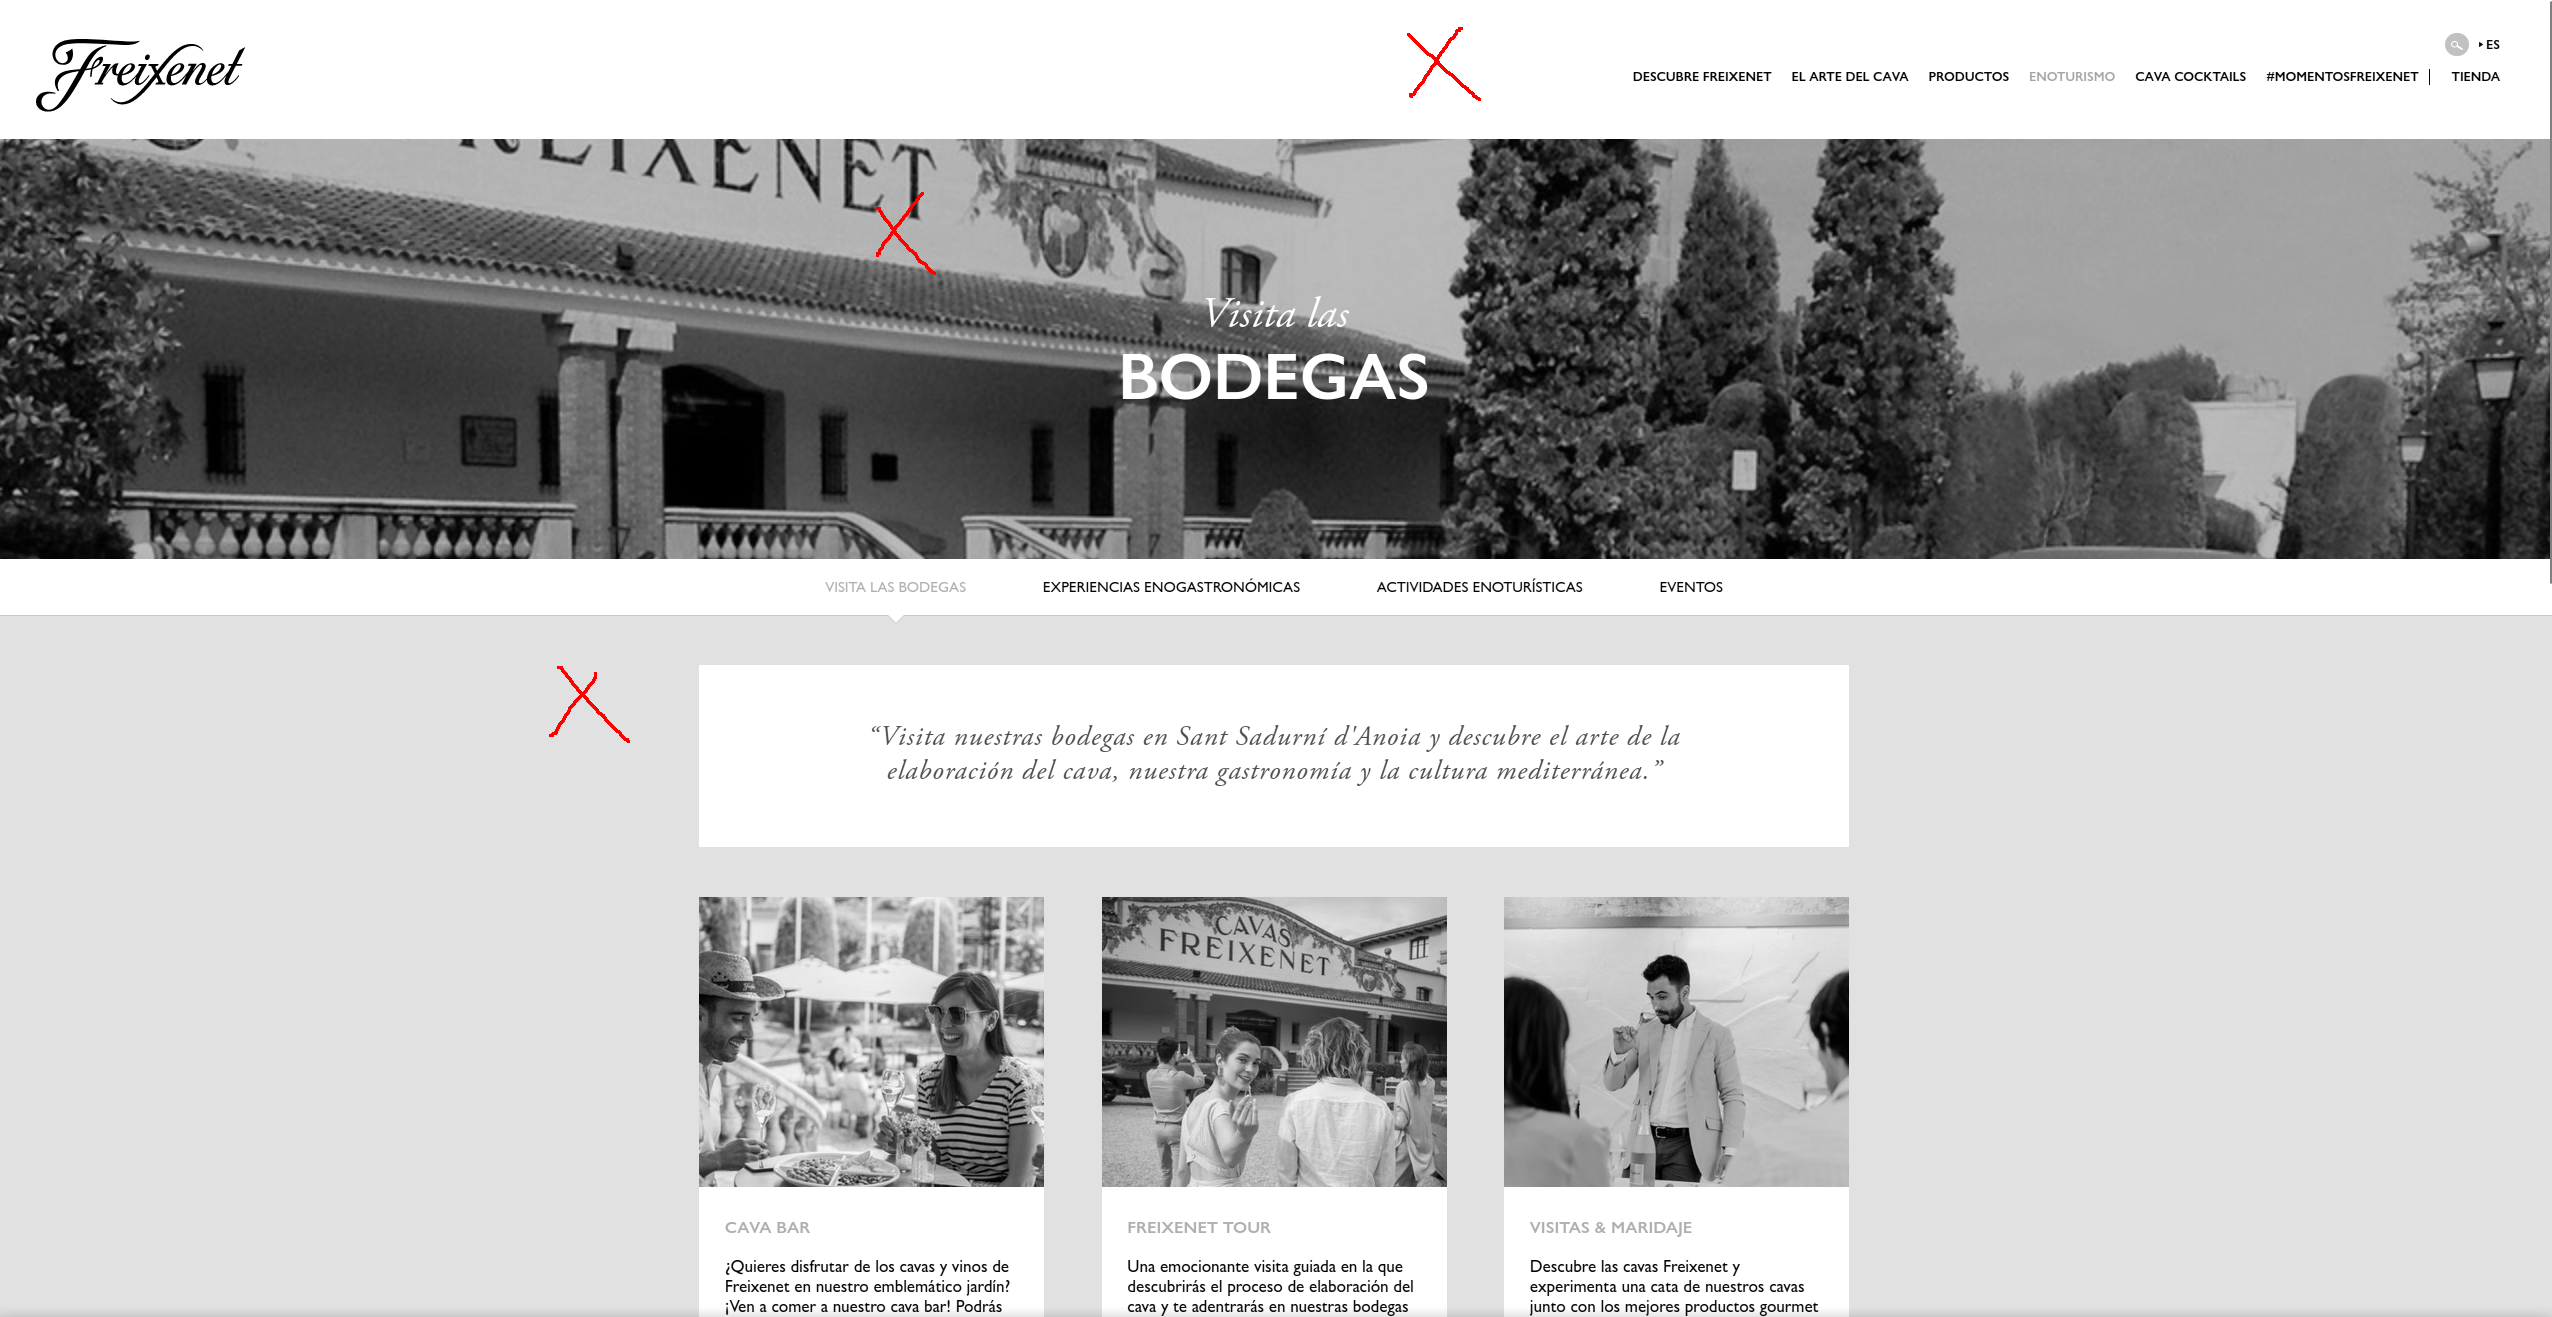
\includegraphics[scale=.1]{../img/3.png}
\end{center}

\subsubsection{¿En qué sección principal se encuentra esta página?}

\begin{center}
        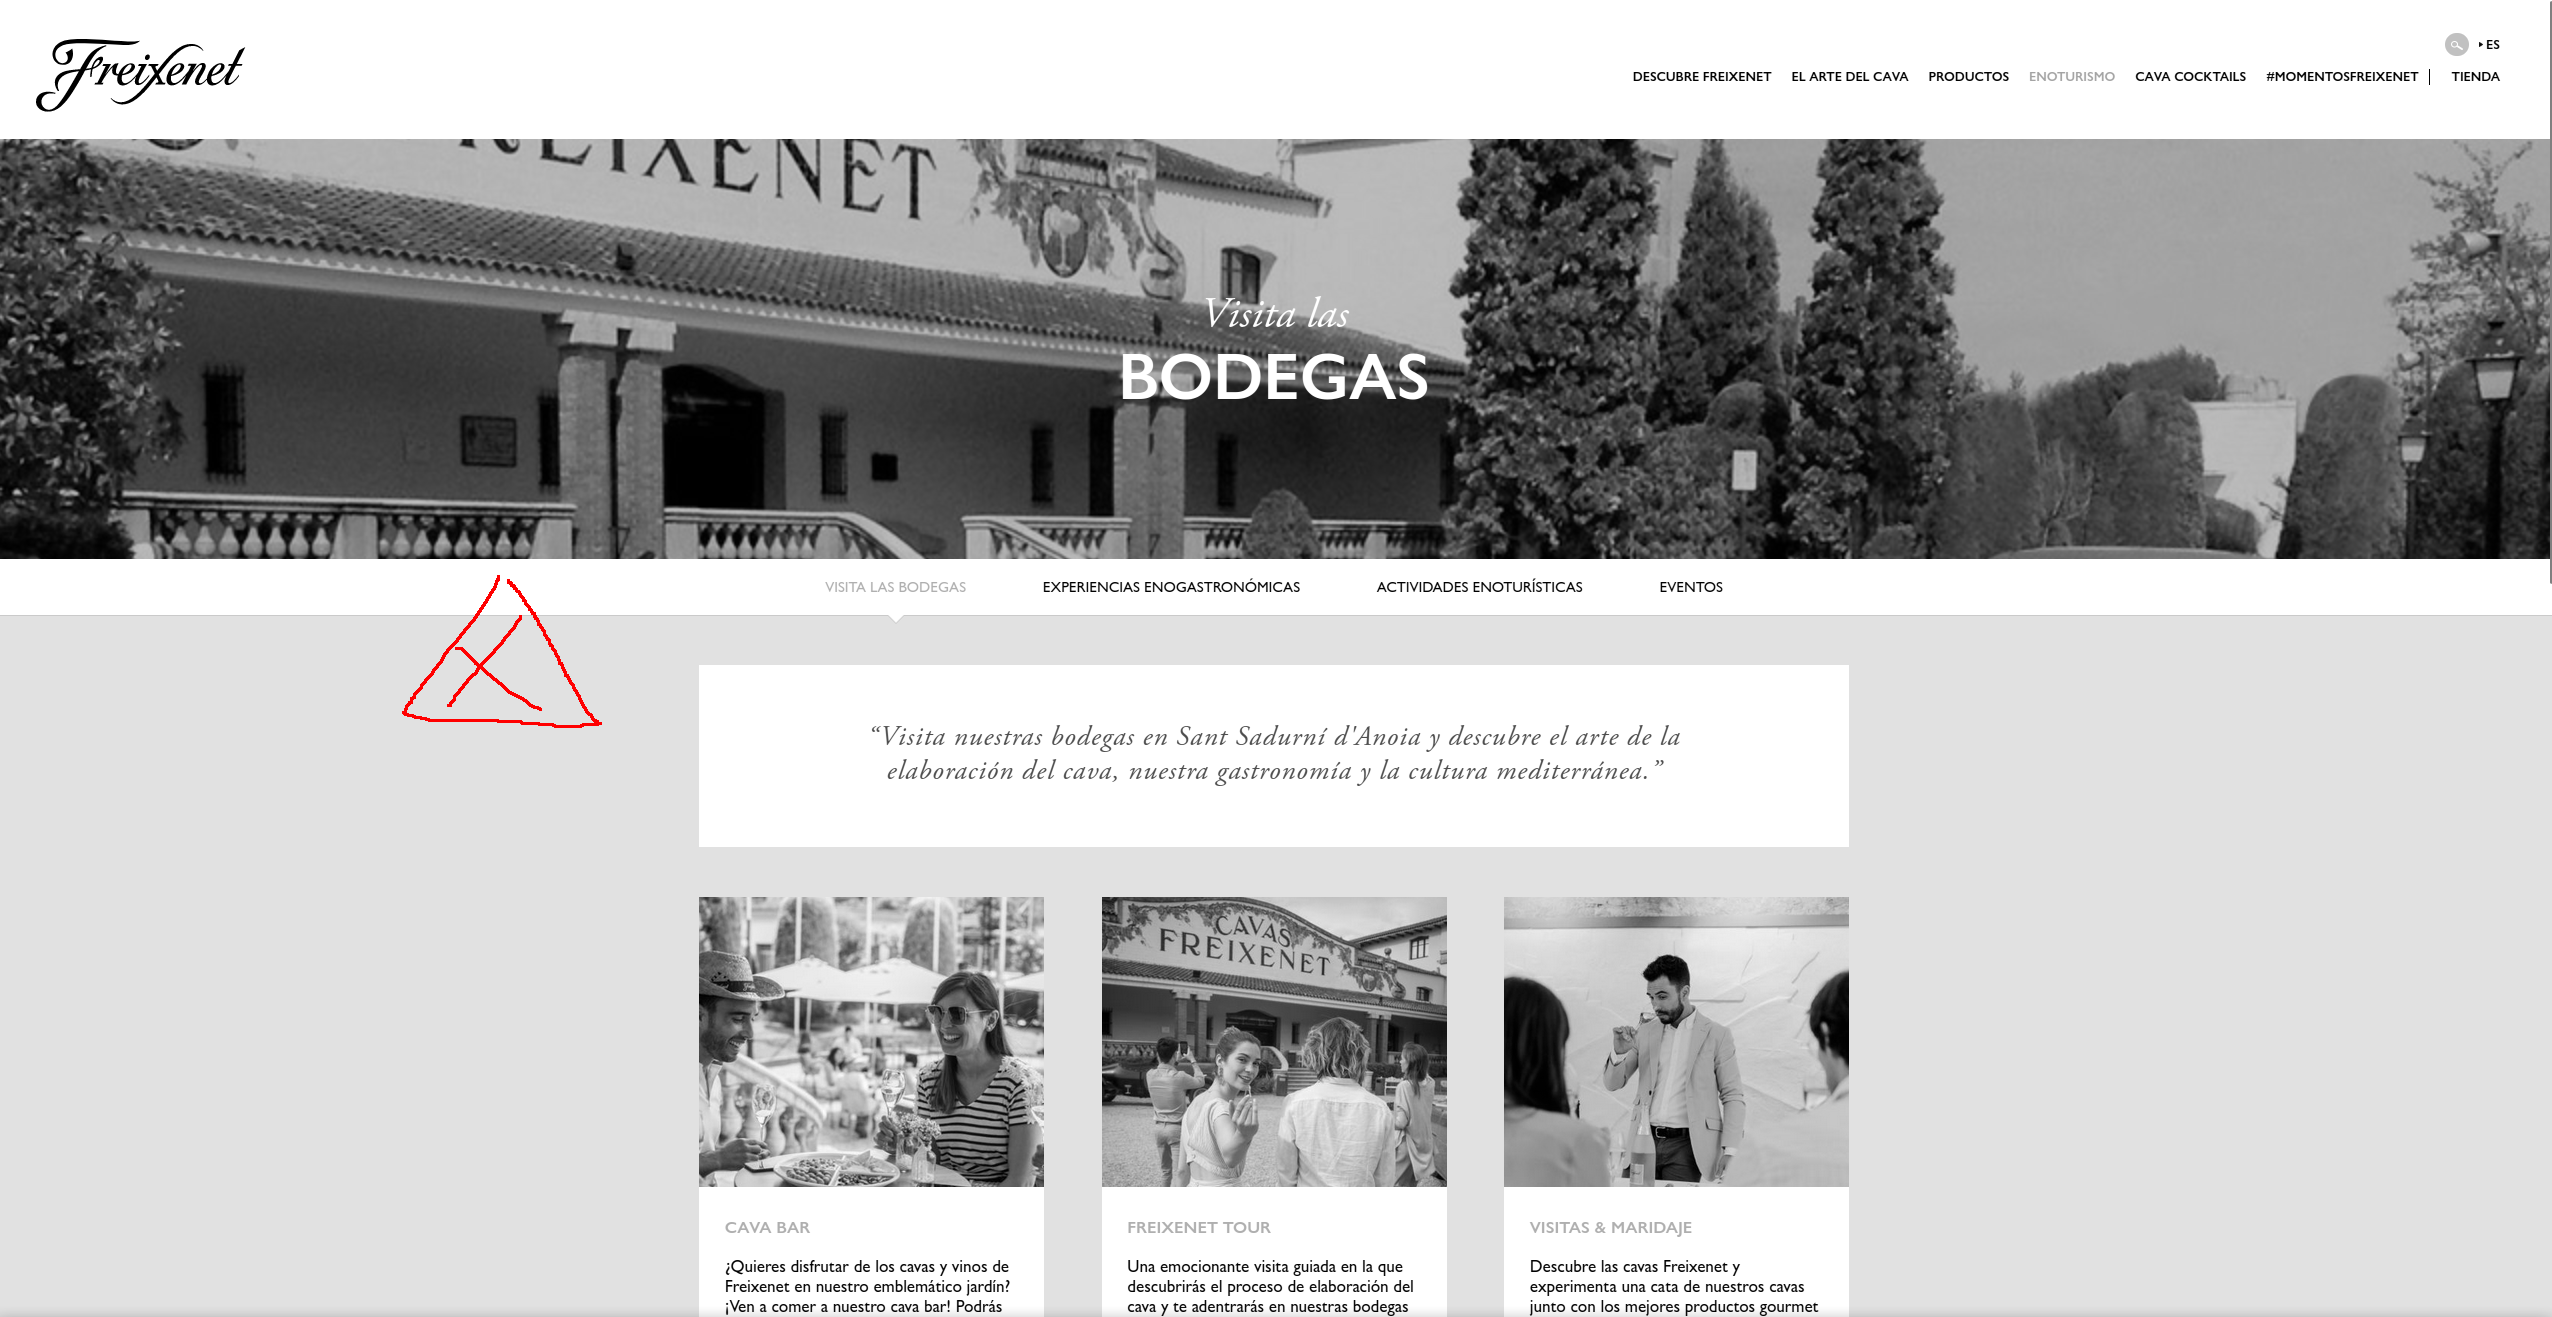
\includegraphics[scale=.1]{../img/4.png}
\end{center}

\subsubsection{¿Qué hay un nivel por encima de aquí?}

\begin{center}
        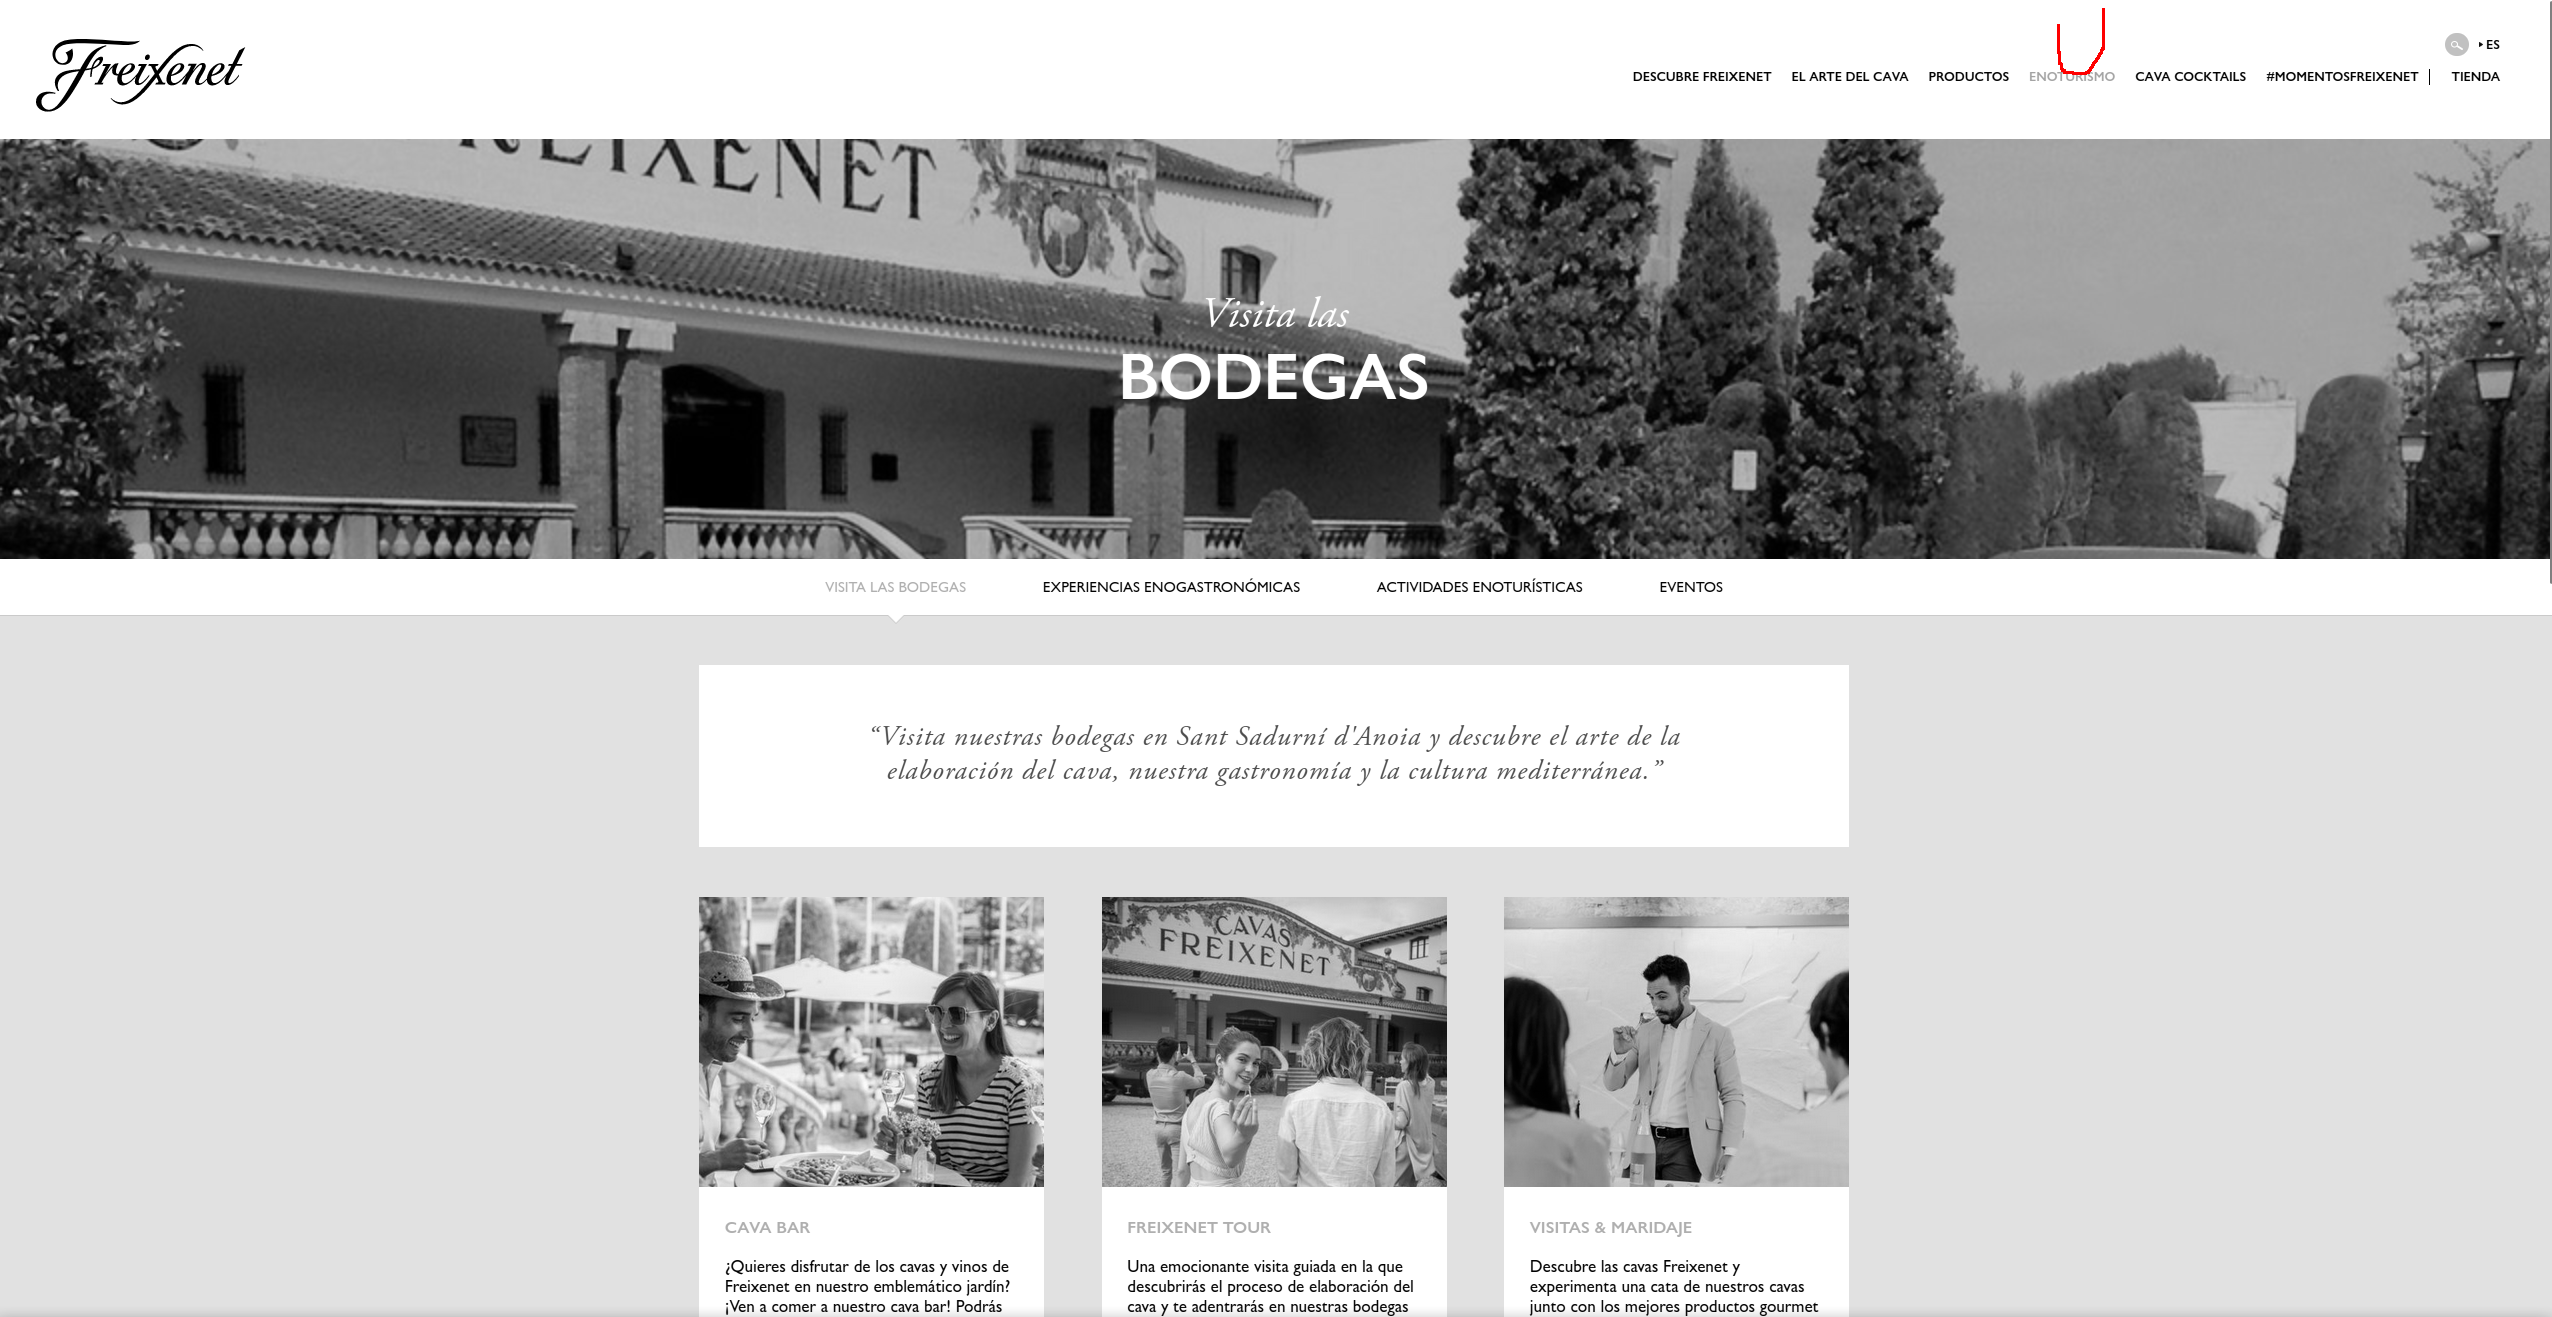
\includegraphics[scale=.1]{../img/5.png}
\end{center}

\subsubsection{¿Cómo llego a la página principal desde aquí?}

\begin{center}
        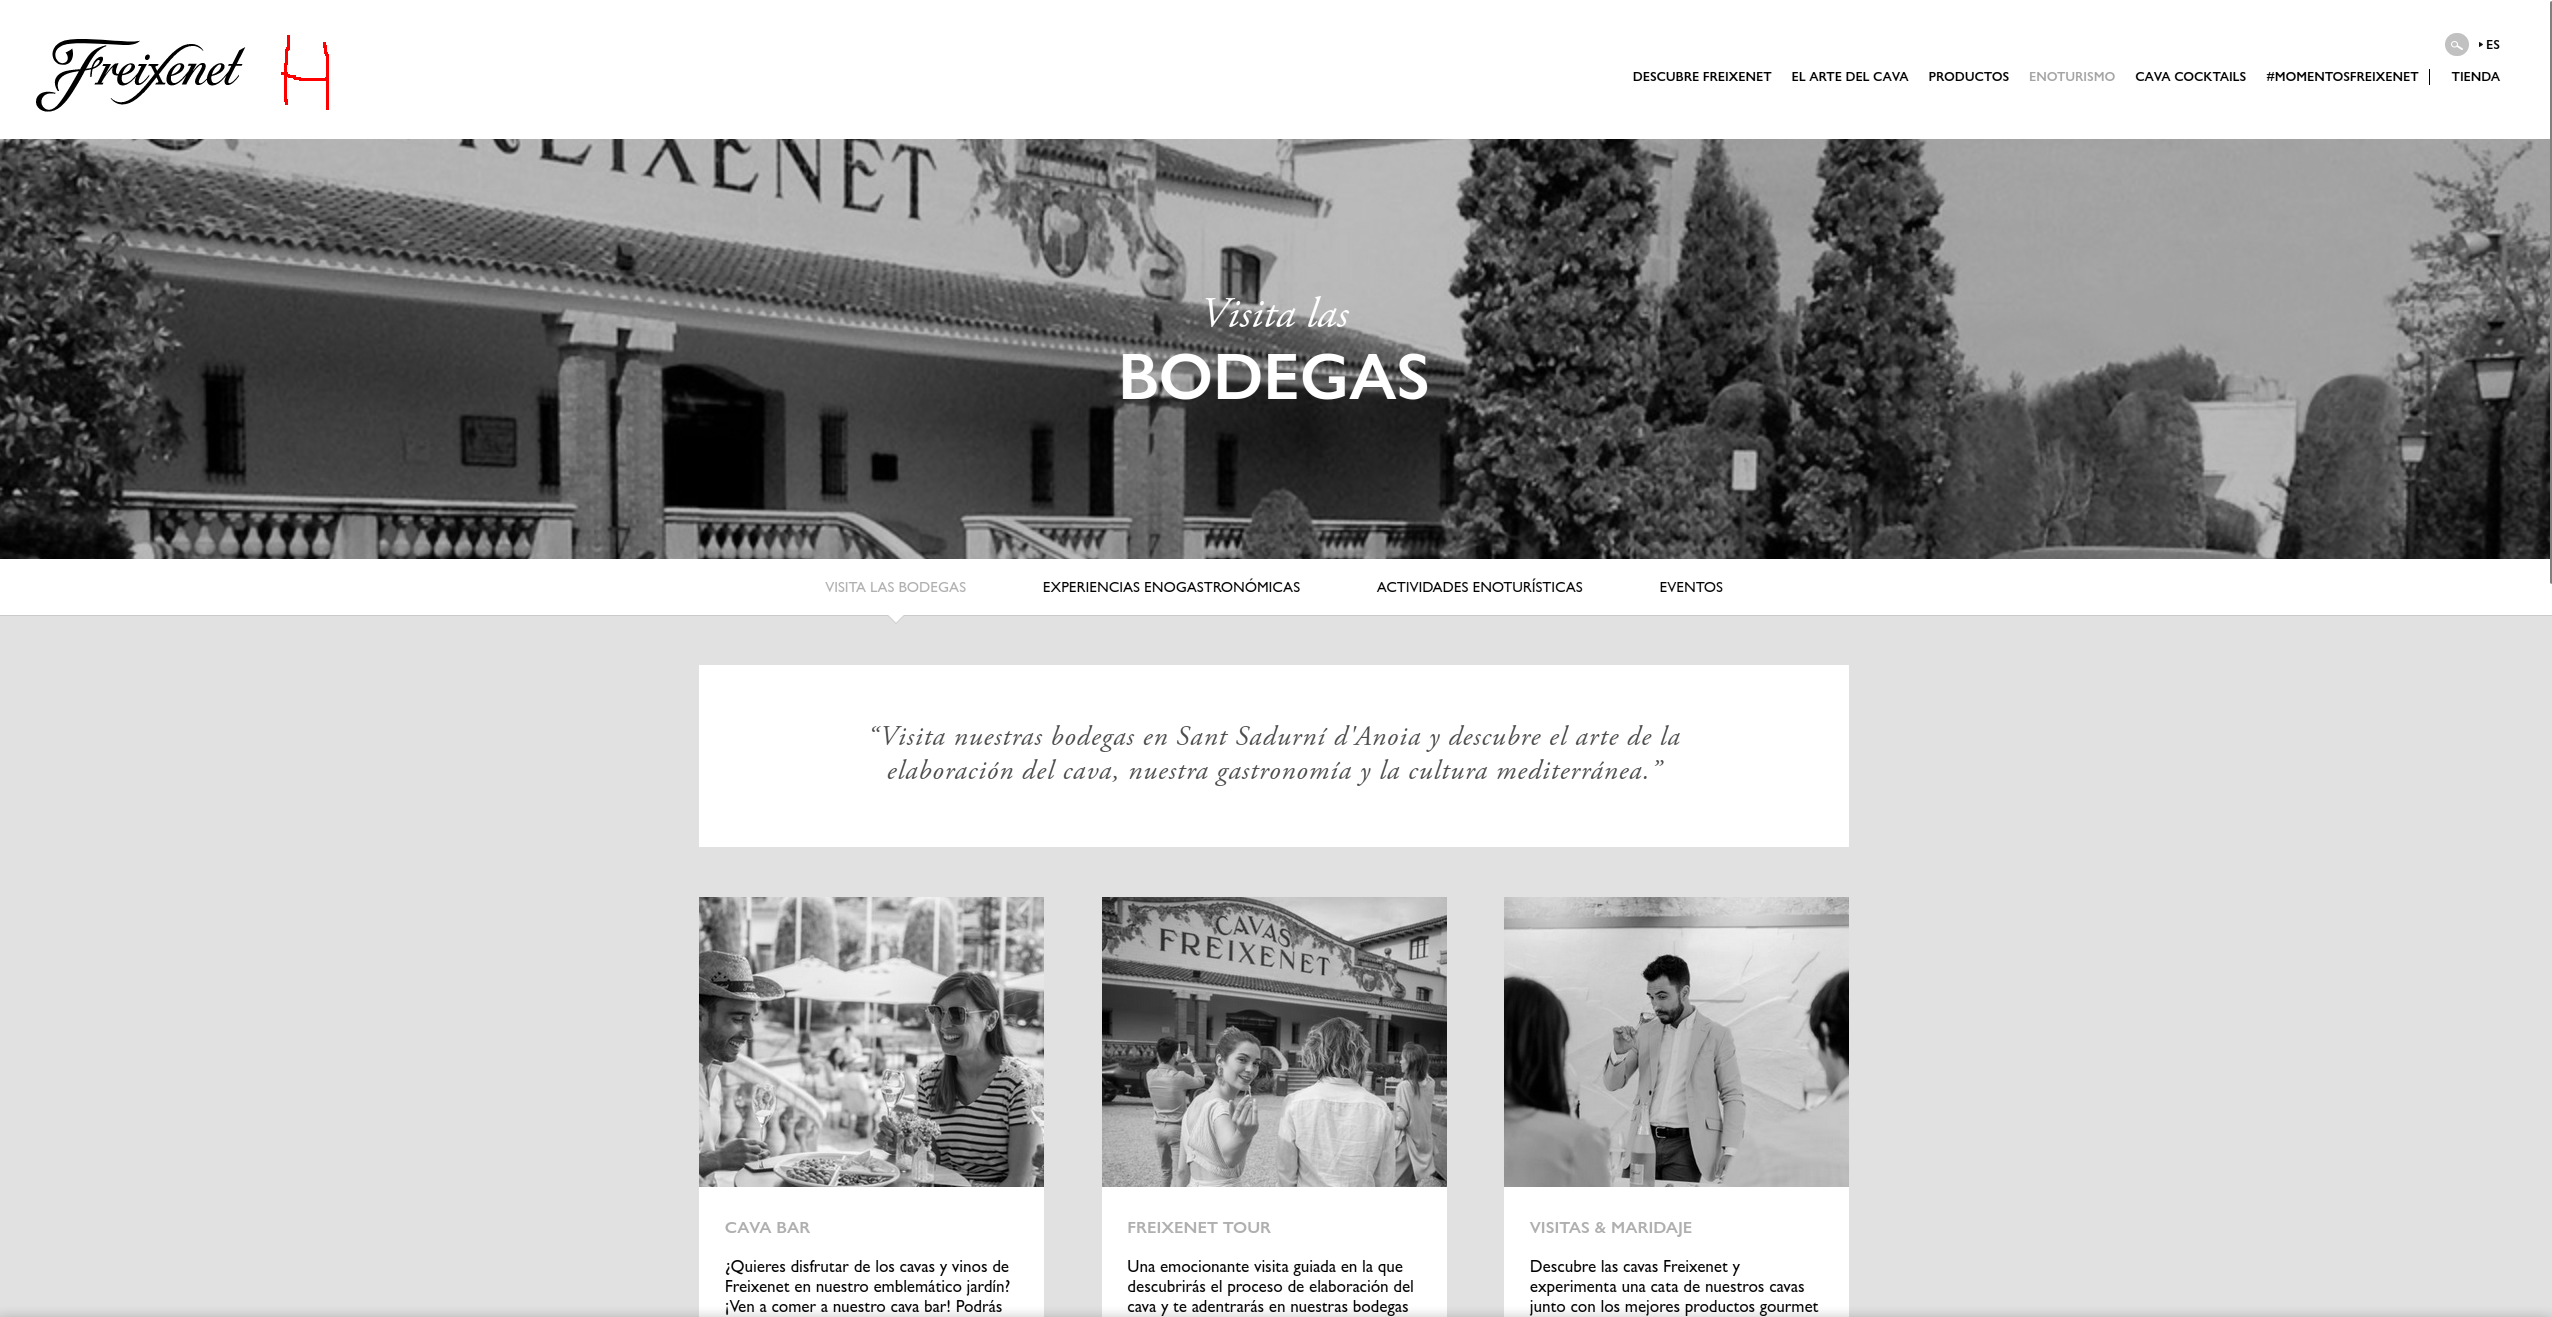
\includegraphics[scale=.1]{../img/6.png}
\end{center}

\subsubsection{¿Cómo llego a la sección superior de esta página?}

\begin{center}
        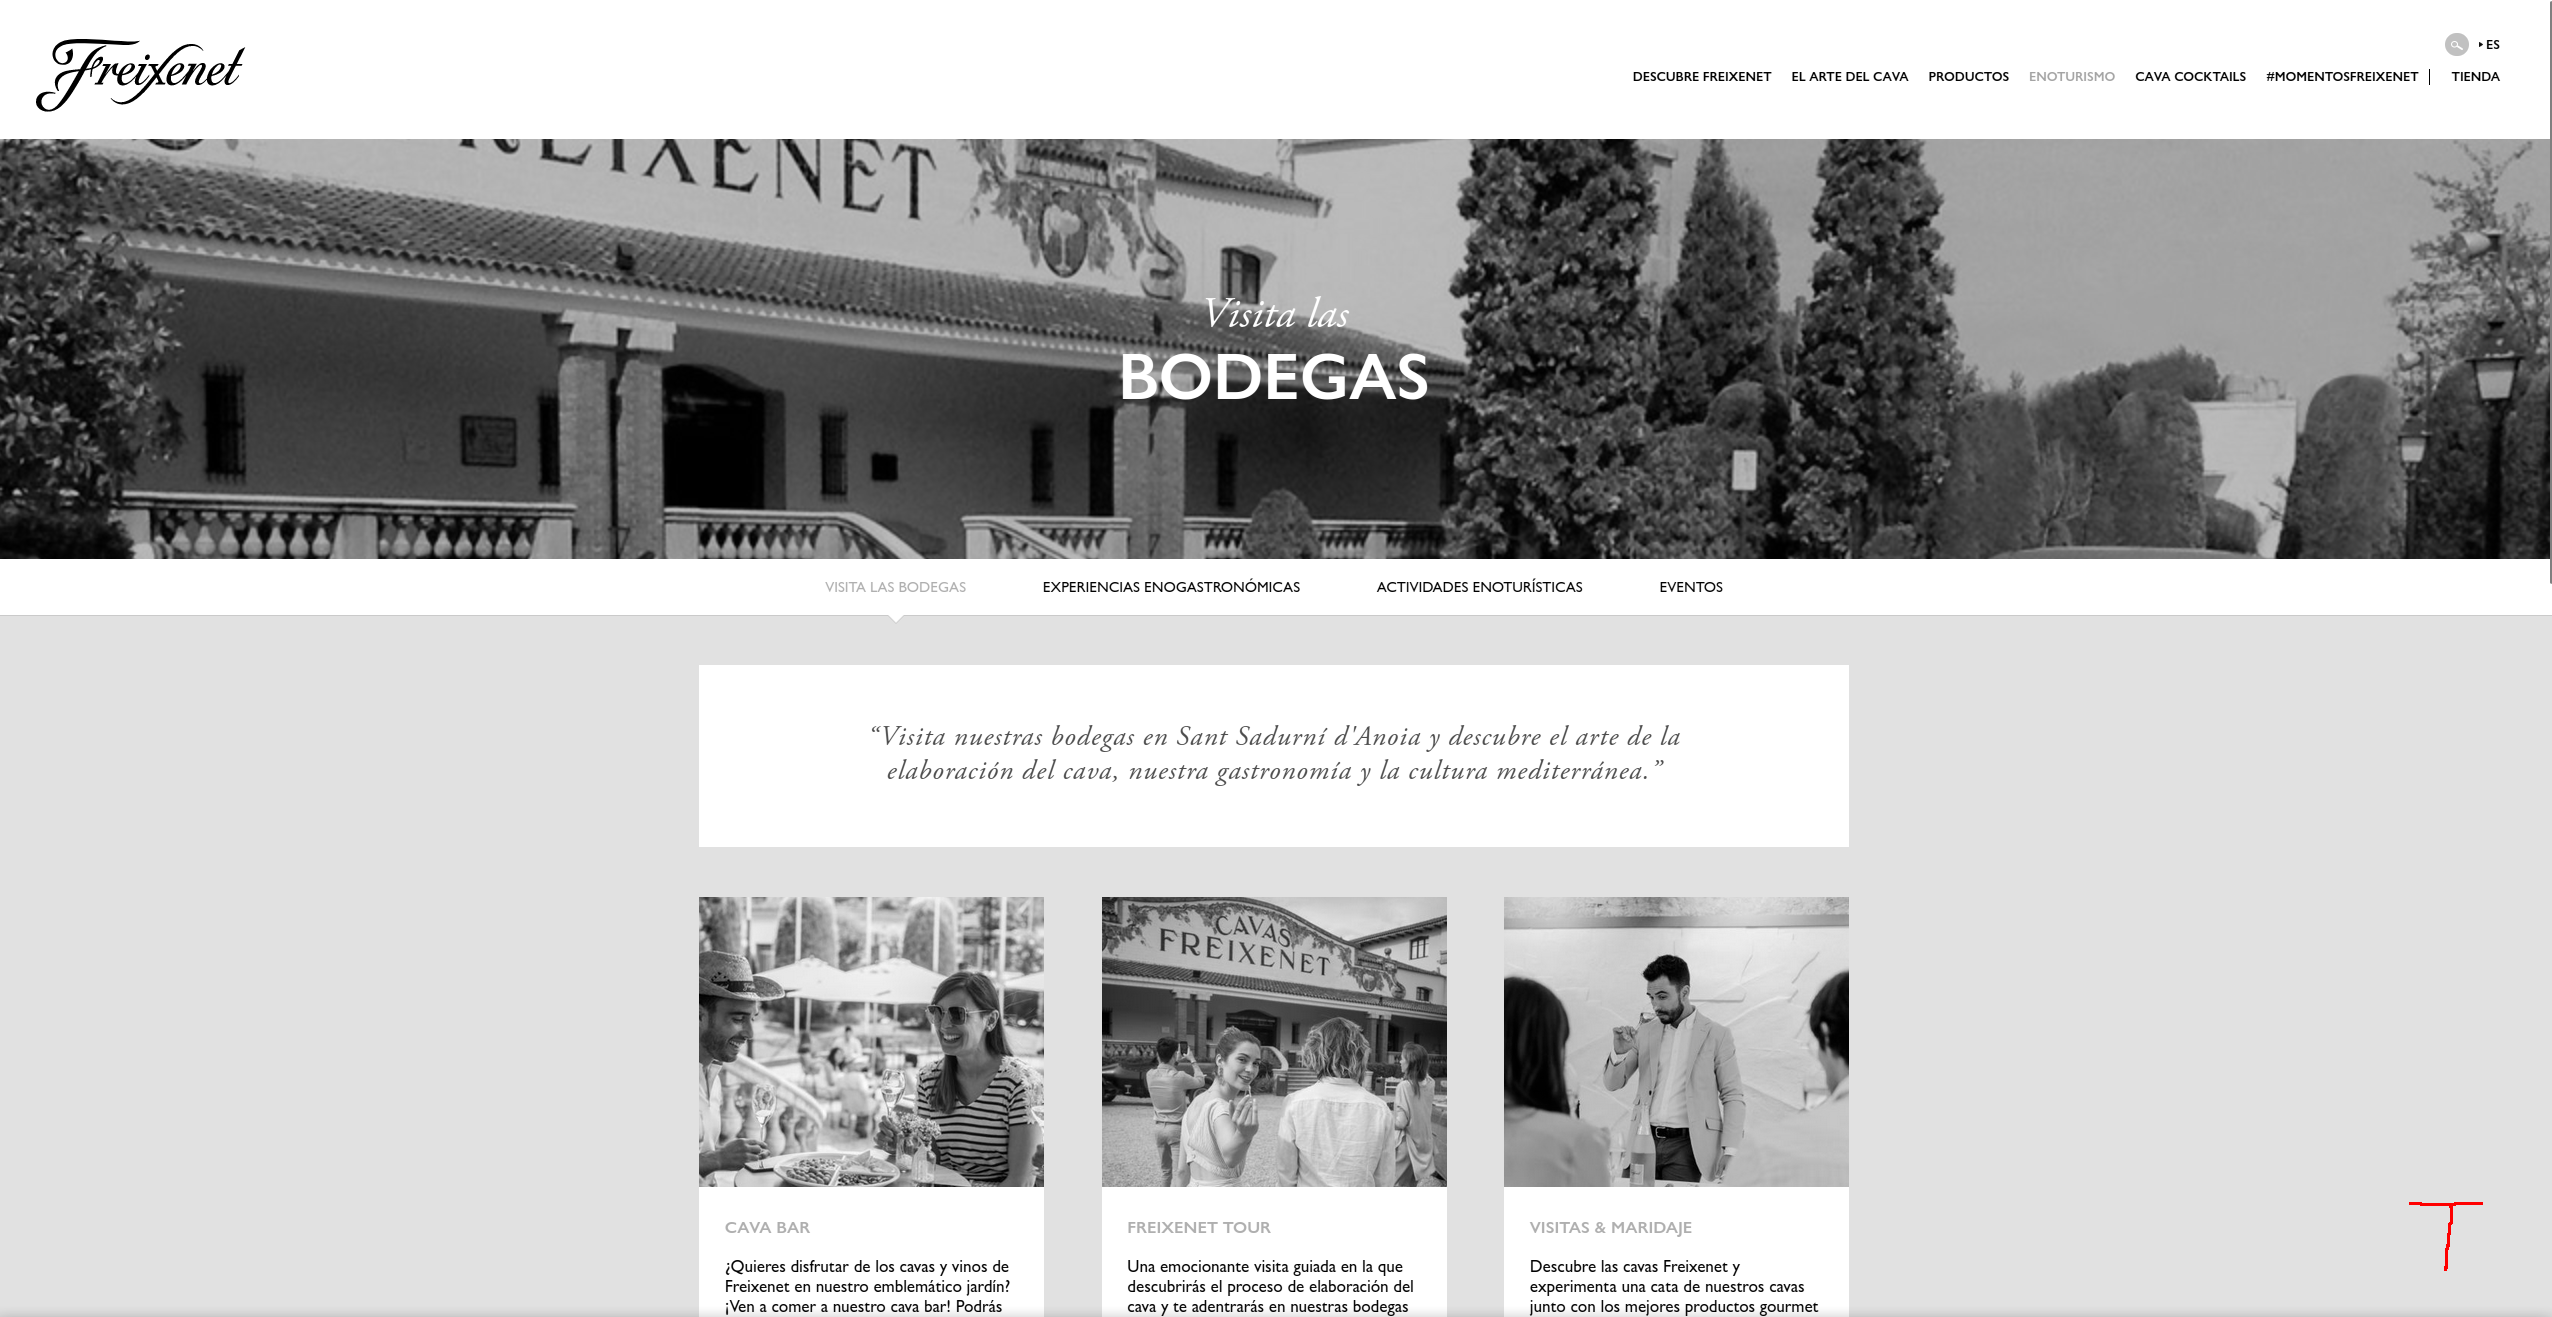
\includegraphics[scale=.1]{../img/7.png}
\end{center}

\subsubsection{¿Qué representa cada grupo de enlaces?}

\begin{center}
        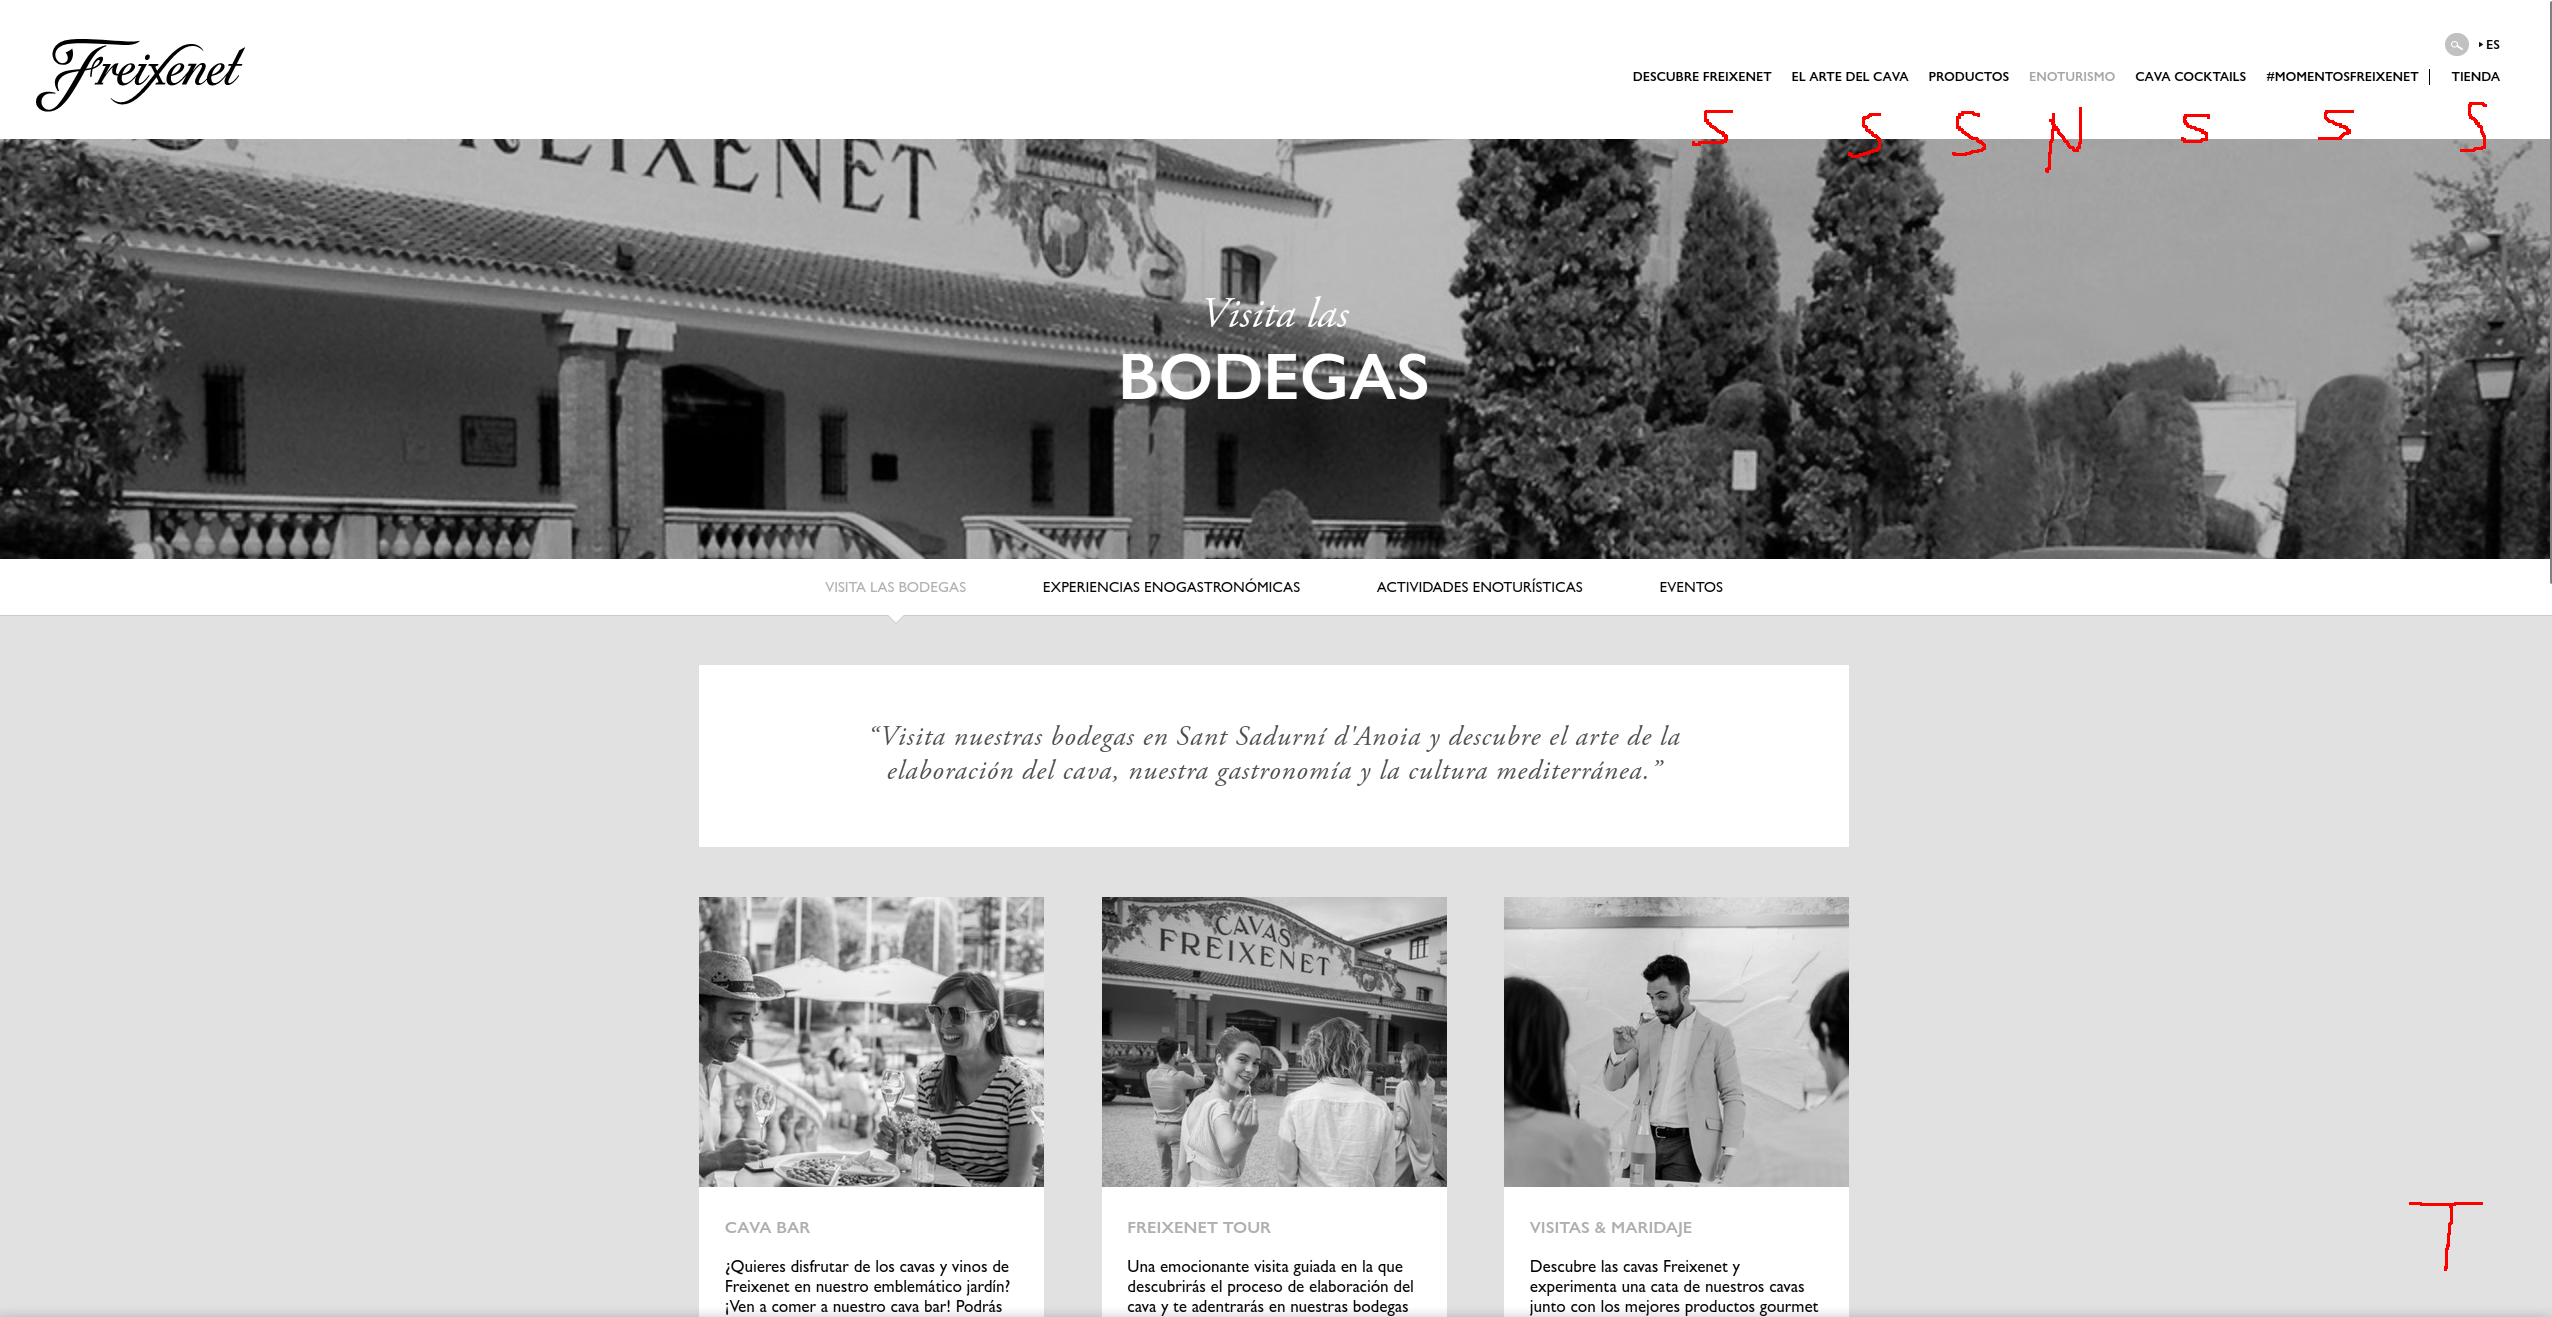
\includegraphics[scale=.1]{../img/8.png}
\end{center}

\subsubsection{¿Cómo llegarías a esta página desde la página principal?}

\begin{center}
        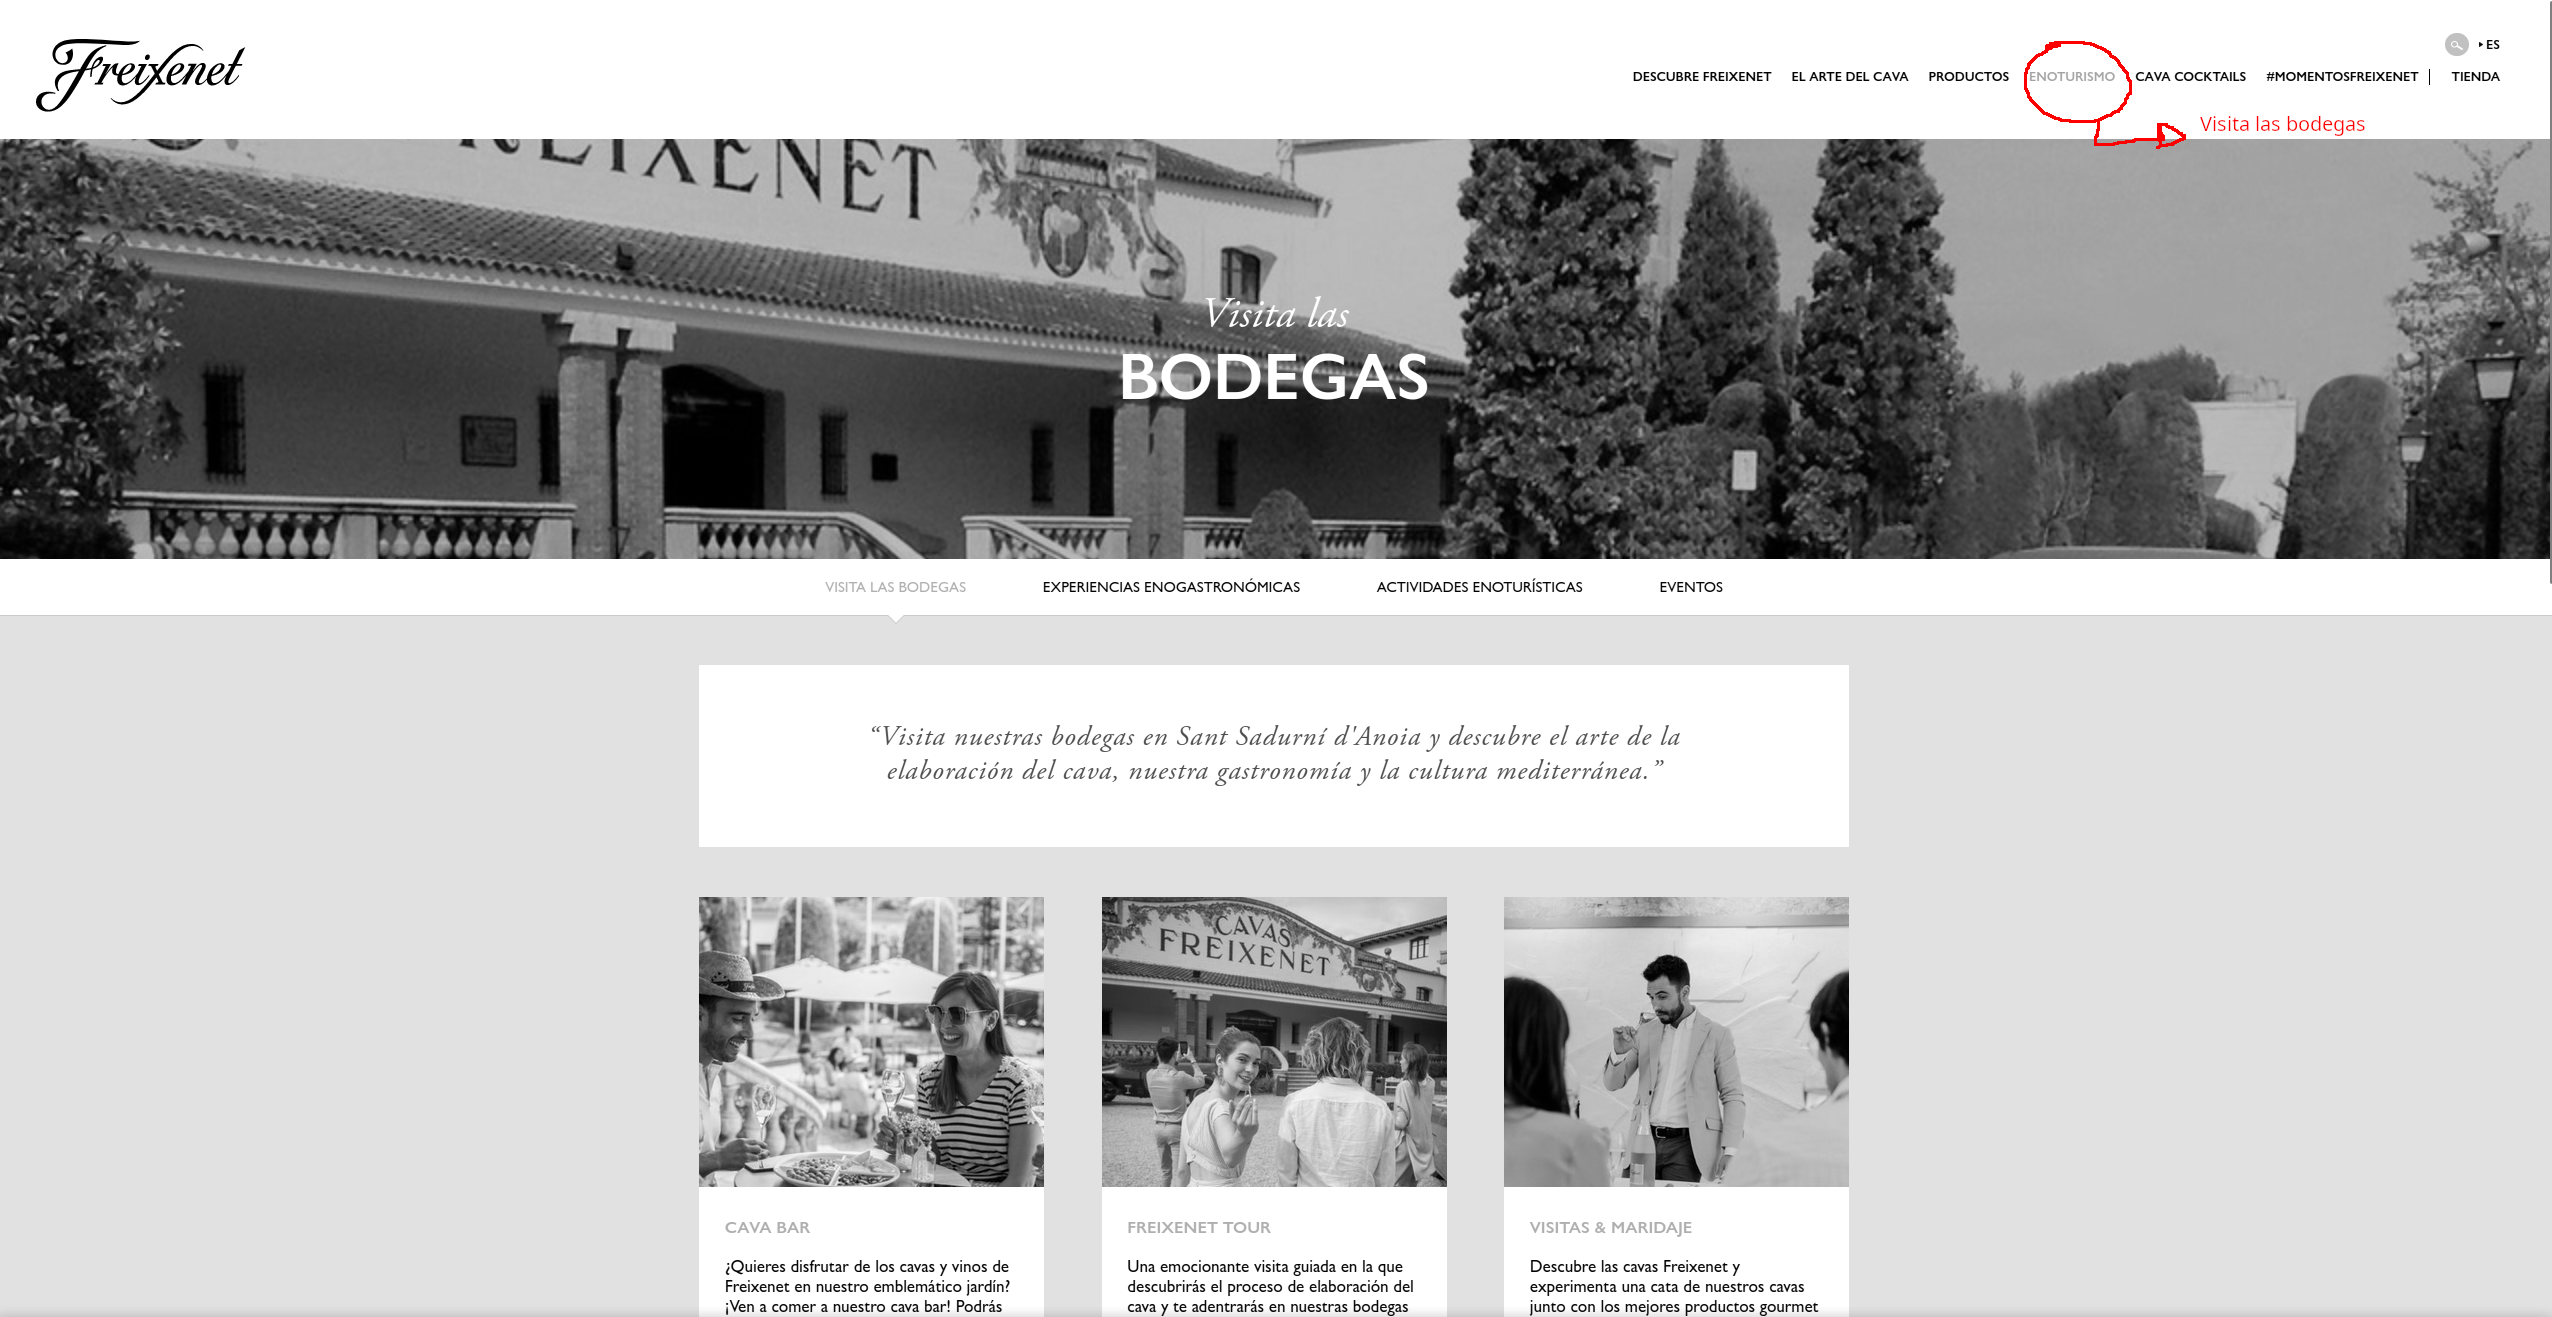
\includegraphics[scale=.1]{../img/9.png}
\end{center}

\newpage

\begin{thebibliography}{X}

\item \textit{Design Toolkit | Accesibilidad.} (n.d.). Fundación UOC. Octubre
2023, de http://design-toolkit.recursos.uoc.edu/es/accesibilidad/

\item \textit{Design Toolkit | Evalación heurística.} (n.d.). Fundación UOC.
Octubre 2023, de http://design-toolkit.recursos.uoc.edu/es/evaluacion-heuristica/

\item \textit{Initiative, W. W. A. (n.d.). Easy Checks – A First Review of Web
        Accessibility.} Web Accessibility Initiative (WAI).
https://www.w3.org/WAI/test-evaluate/preliminary/

\item \textit{Keith Instone | Navigation stress test.} (n.d.). Keith Instone.
        Octubre 2023, de http://instone.org/navstress/

\end{thebibliography}

\end{document}
